\chapter[Tranças e a Teoria dos Nós]{Tranças e a Teoria dos Nós}
\label{cap-5}
\chaptermark{}
%
\hfill%
\begin{minipage}{10cm}
\begin{flushright}
\rightskip=0.5cm
\textit{``As far as the laws of mathematics refer to reality, they are not certain, and as far as they are certain, they do not refer to reality.''}
\\[0.1cm]
\rightskip=0.5cm
--- Albert Einstein
\end{flushright}
\end{minipage}

\section{Conexões entre tranças e nós}

    Vamos agora discutir algumas conexões entre tranças e a teoria dos nós.
    
	\par\vspace{0.3cm} Resumidamente, um nó é uma curva poligonal simples fechada em $\mathbb{R}^3$, 
	mas para os propósitos deste texto poderemos pensar em um nó como sendo uma curva suave simples, 
	como os diagramas da Figura \ref{exemplos de nos}.
	
	\par\vspace{0.3cm} Os nós (ou, de modo mais geral, \textit{links}) e as tranças possuem semelhanças. 
	Por exemplo, ambos são definidos em termos de figuras de cordas no espaço tridimensional, e ambos 
	têm uma noção de equivalência, geralmente chamada de isotopia, que descreve quando duas figuras 
	são equivalentes, ou seja, quando duas figuras representam o mesmo nó ou a mesma trança.  
	%
	\begin{figure}[H]
	\begin{center}
		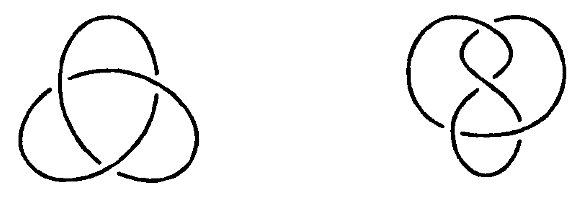
\includegraphics[width=7cm]{Images/exemplos_de_no.png}
	\end{center}\caption{Exemplos de nós}
	\label{exemplos de nos}
	\end{figure}
	%
	\par\vspace{0.3cm} É claro que há algumas diferenças, a principal delas sendo o fato de que 
	as tranças têm extremidades que não podem se mover durante isotopias, i.e., as extremidades 
	ficam fixas conforme deformamos a trança, como vimos nas seções anteriores. Outra diferença 
	é que cada corda de uma trança vai monotonicamente da esquerda para a direita, enquanto que 
	não há essa restrição em relação aos \textit{links}.
	
	\par\vspace{0.3cm} Na verdade, uma das primeiras motivações para o estudo das tranças era ajudar 
	a entender a teoria dos nós e \textit{links}. A conexão é que toda trança pode ser ``fechada'' 
	para formar um \textit{link}. Era esperado que a estrutura de grupo nas tranças levasse a algum 
	tipo de estrutura de grupo no conjunto de \textit{links}, mas isso não acontece. Não obstante, 
	há outras maneiras de usar tranças para ajudar com o estudo de \textit{links}.
	
	\par\vspace{0.3cm} Mas como formamos um \textit{link} a partir de uma trança? Fácil: basta 
	ligar as extremidades sem introduzir novos cruzamentos.
	
	\par\vspace{0.3cm} Assim como fizemos para as tranças, também é possível alterar diagramas de 
	nós através de deformações (ou movimentos) elementares (e seus respectivos inversos). 
	Esses movimentos são chamados de \textit{movimentos de Reidemeister}, classificados em 3 tipos.
	%
	\begin{figure}[H]
		\begin{center}
			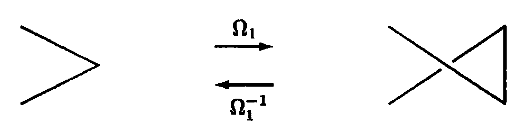
\includegraphics[width=10cm]{Images/reidemeister_1.png}
		\end{center}\caption{Movimento de Reidemeister do tipo I}
		\label{reidemeister tipo 1}
	\end{figure}
	%
	\begin{figure}[H]
		\begin{center}
			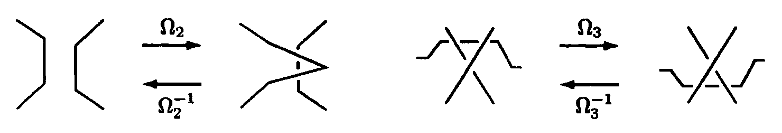
\includegraphics[width=14cm]{Images/reidemeister_2_e_3.png}
		\end{center}\caption{Movimentos de Reidemeister dos tipos II e III}
		\label{reidemeister tipos 2 e 3}
	\end{figure}
	%
	O teorema a seguir, que não será demonstrado, nos dá os análogos, para nós e \textit{links}, 
	das relações de trança.
	%
	\begin{theorem}
	\label{equivalencia de nos}
		Seja $K$ um nó (ou \textit{link}) e suponha que $D$ e $D'$ são dois diagramas de nó de $K$. 
		Então, $D$ pode ser deformado em $D'$ através de uma sequência finita de movimentos de 
		Reidemeister, ou seja, através de uma sequência finita das deformações 
		$\Omega_1^{\pm1}, \Omega_2^{\pm1}$ e $\Omega_3^{\pm1}$. 
	\end{theorem}  
	%
	O Teorema \ref{equivalencia de nos} nos dá um algoritmo conceitualmente muito simples 
	para verificar se dois diagramas são, de fato, equivalentes, i.e., representam o mesmo nó: 
	basta tentar todas as sequências possíveis de movimentos em um dos diagramas e ver se o outro 
	diagrama é produzido em alguma dessas sequências. Esse método de tentativa é válido pois 
	recentemente foi provado que, dados dois diagramas, se um deles pode ser deformado no outro, 
	ou seja, se eles representam o mesmo nó, então a quantidade de movimentos é limitada superiormente 
	por uma função do número de cruzamentos no diagrama. Contudo, como esse limite superior é extremamente
	grande \cite{limite-superior-1, limite-superior-2, limite-superior-3}, esse algoritmo ainda não é prático.
	Ainda assim, os movimentos de Reidemeister são úteis para vários propósitos teóricos, como estabelecer 
	vários invariantes de nós.
	
	\par\vspace{0.3cm} Os movimentos de Reidemeister, definidos para nós e \textit{links}, possuem 
	análogos para as tranças. Esses análogos são os próprios movimentos de Reidemeister, com exceção 
	do tipo I, uma vez que cada corda da trança deve ser monotônica. Isso significa que nunca podemos 
	fazer um movimento do tipo I, pois não podemos ter \textit{loops}.
	
	\par\vspace{0.3cm} Mas e os movimentos tipo II? Se, na trança, há uma parte que parece com o diagrama à
	esquerda da Figura \ref{identidade b2}, então podemos endireitar ambas as cordas: esse é um movimento 
	tipo II. Algebricamente, ele corresponde a cancelar $\sigma_i\sigma_i^{-1}$ (ou $\sigma_i^{-1}\sigma_i$) 
	em uma palavra, o que é claro que podemos fazer. Também podemos sempre inserir tais pares sempre que
	quisermos, sem alterar a trança.
	
	\par\vspace{0.3cm} E os movimentos tipo III? Observe a Figura \ref{trancas equivalentes}: 
	ela é um movimento de Reidemeister tipo III!
	
	\par\vspace{0.3cm} De forma análoga ao Teorema \ref{equivalencia de nos}, por meio de uma 
	sequência de movimentos de Reidemeister dos tipos II e III, podemos partir de um diagrama 
	de uma trança e chegar em qualquer outro diagrama de uma trança equivalente. 
	Note, em particular, que esses movimentos (tipo II e tipo III) não alteram a paridade do 
	número de cruzamentos.
	
	\par\vspace{0.3cm} Voltando às conexões entre tranças e \textit{links} (e nós), lembre-se 
	do que foi dito no início da seção: que fechando uma trança, obtemos um \textit{link}. 
	De fato, não só podemos obter \textit{links} (e nós) a partir de tranças, como também 
	podemos obter \textbf{todos} os \textit{links} a partir de tranças, como diz o seguinte 
	teorema, que não será demonstrado aqui.
	%
	\begin{theorem}[Alexander]
	\label{teorema de Alexander}
		Qualquer nó ou link $K$ pode ser representado como uma trança fechada.
	\end{theorem}
	%
	Uma consequência boa do Teorema \ref{teorema de Alexander} é que temos uma maneira direta de 
	descrever qualquer nó (e \textit{link}) sem precisar fazer um desenho. Em vez de dizer 
	``é o nó que vai por cima, depois por baixo, e volta por trás para onde estava antes só que 
	do outro lado e$\dots$'', o que tem desvantagens óbvias, podemos simplesmente dizer ``é o nó 
	que obtemos fechando a trança de 3 cordas $\sigma_1\sigma_2^{-1}\sigma_1\sigma_2^2\sigma_1^2\sigma_2^3$''.
	Muito mais simples.
	
	\par\vspace{0.3cm} Contudo, o Teorema \ref{teorema de Alexander} não nos dá uma correspondência 
	única entre tranças e \textit{links}. Várias tranças diferentes podem ser fechadas no mesmo 
	\textit{link} e pode até ser o caso de que tranças com quantidades de cordas diferentes 
	fechem no mesmo \textit{link}, como mostra a figura a seguir.
	%
	\begin{figure}[H]
		\begin{center}
			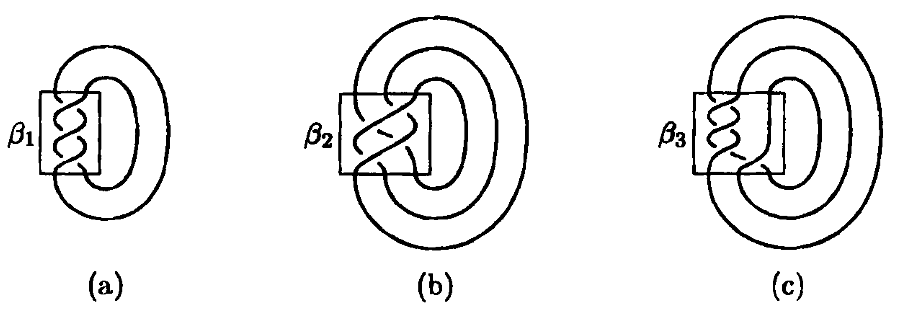
\includegraphics[width=12cm]{Images/fechamento_de_trancas_em_nos.png}
		\end{center}\caption{Tranças não equivalentes que fecham em nós equivalentes.}
		\label{fechamento de trancas em nos}
	\end{figure}
	%
	Quando dois nós (ou \textit{links}) podem ser deformados um no outro, dizemos que eles 
	são \textit{equivalentes} ou \textit{isotópicos}. Por exemplo, todas as tranças de 
	$B_2(\mathbb{R}^2)$ (ou seja, todas as tranças de duas cordas) são fechadas no 
	mesmo nó: o trivial.
	
	\par\vspace{0.3cm} Logo, se queremos estudar teoria dos nós via teoria das tranças, 
	precisamos de um método para determinar se duas tranças fechadas são equivalentes, 
	ou seja, se dois \textit{links} são isotópicos. De fato, a resposta para essa pergunta 
	está no chamado \textit{teorema de Markov}, que será enunciado mais à frente.
	
	\par\vspace{0.3cm} Outro fato importante é que invariantes de trança podem não ser invariantes 
	na trança fechada associada. Por exemplo, sabemos que dada uma trança $\beta$, $l$ 
	(o homomorfismo de comprimento) é um invariante de $\beta$. Contudo, $l$ não precisa 
	ser um invariante de $\widetilde{\beta}$, a trança fechada associada a $\beta$. 
	Por exemplo, na Figura \ref{fechamento de trancas em nos} $l(\beta_1) = 3 \neq 4 = l(\beta_2)$, mas
	$\widetilde{\beta_1}\sim\widetilde{\beta_2}$, i.e., os seus fechamentos são nós equivalentes.
	
	\par\vspace{0.3cm} Isso suscita a seguinte questão: existe um invariante de nó 
	da trança fechada $\widetilde{\beta}$ que é definido a partir de um invariante da trança $\beta$?
	
	\par\vspace{0.3cm} A resposta é sim. Consideremos a permutação $\pi(\beta)$ associada 
	à trança $\beta$. Sabemos que $\pi(\beta)$ pode ser expressa como produto de transposições, a saber
	%
	\begin{align*}
	    \pi(\beta) = C_1\cdots C_k.
	\end{align*}
	%
	Então $k$, que denotaremos por $\mu(\beta)$, é o número de componentes de $\widetilde{\beta}$ 
	e um invariante do link $\widetilde{\beta}$, uma vez que o seguinte é válido:
	%
	\begin{align*}
	    \beta\sim\beta' \Rightarrow \pi(\beta) = \pi(\beta') \Rightarrow \mu(\beta) = \mu(\beta').
	\end{align*}
	%
	Portanto, $\widetilde{\beta}$ é um nó se, e somente se, $\pi(\beta)$ é um ciclo de ordem $n$, 
	isto é, $\pi(\beta)$ não deixa pontos fixos. Nesse caso, dizemos que $\beta$ é uma 
	trança fechada de um componente. Como um ciclo de ordem $n$ é escrito por um produto 
	de $n-1$ transposições, então $\widetilde{\beta}$ é um nó se, e só se, $k = n-1$.
	
	\par\vspace{0.3cm} Note também que da maneira que definimos $\mu(\beta)$, é claro que, 
	escrevendo $\beta = \sigma_{i_1}^{\varepsilon_1}\cdots\sigma_{i_k}^{\varepsilon_k}$, 
	sendo $\varepsilon_i = \pm1$, temos como consequência imediata o fato de que 
	$\mu(\beta) = \displaystyle{\sum_{i}^{k}|\varepsilon_i|}$.
	
	\par\vspace{0.3cm} Até agora, vimos que a toda trança podemos associar um \textit{link}, 
	mas que essa correspondência não é única (veja a Figura \ref{fechamento de trancas em nos}). 
	Esse fato levanta a questão: é possível dizer quando que o fechamento de duas tranças não 
	equivalentes nos dá o mesmo \textit{link}?
	
	\par\vspace{0.3cm} A resposta (em parte) é sim, contida no \textit{teorema de Markov} 
	(ainda que não tenha sido o próprio Markov quem demonstrou). Mas o quê exatamente é o teorema de Markov?
	
	\par\vspace{0.3cm} Primeiro, vamos observar alguns fatos, como o lema a seguir.
	%
	\begin{lemma}
	\label{conjugacoes dao o mesmo link}
		Sejam $\beta$ e $\gamma$ duas tranças de $n$ cordas. Então, o fechamento de $\beta$ 
		e o fechamento de $\gamma\beta\gamma^{-1}$ nos dão o mesmo \textit{link}.
	\end{lemma}
	%
	\begin{proof}
		A demonstração segue a ideia da Figura \ref{conjugacao nao altera link}. 
		Basicamente, fechando a trança $\gamma\beta\gamma^{-1}$, podemos mover 
		a trança $\gamma^{-1}$ pelo \textit{link} de modo que tenhamos a trança 
		$\beta\gamma^{-1}\gamma$, ou seja, a trança  $\beta$. Observe a figura.
		%
		\begin{figure}[H]
			\begin{center}
				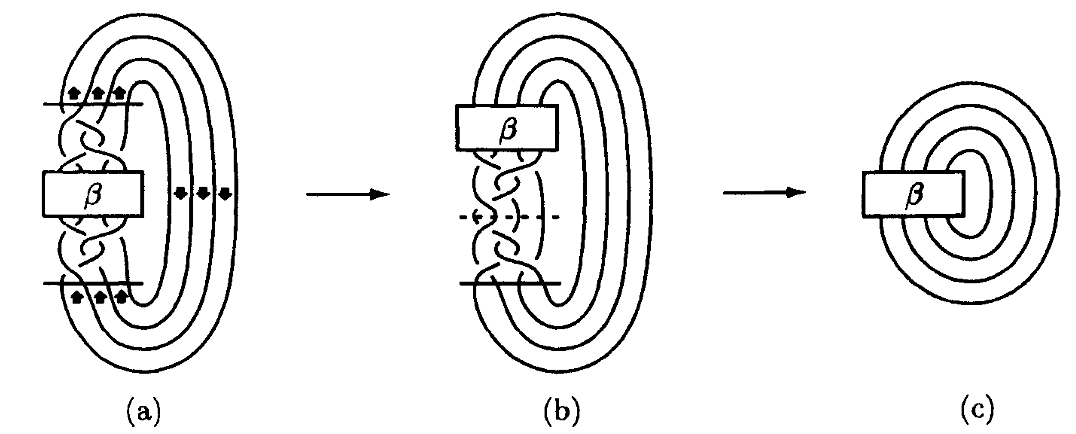
\includegraphics[width=12cm]{Images/conjugacao_nao_altera_link.png}
			\end{center}\caption{Conjugações não alteram o \textit{link}.}
			\label{conjugacao nao altera link}
		\end{figure}
		%
	\end{proof} 
	%
	Por fim, antes de enunciarmos o teorema de Markov, suponha que $\beta$ é um trança de $n$
	cordas e considere $\sigma_n$ um gerador de $B_{n+1}(\mathbb{R}^2)$. De maneira natural, 
	se considerarmos $\beta$ como um elemento de $B_{n+1}(\mathbb{R}^2)$ em vez de $B_n(\mathbb{R}^2)$, 
	podemos definir outras duas tranças de $n+1$ cordas,
	%
	\[
    	\begin{array}{ccc}
    	    \beta' = \beta\sigma_n & \text{e} & \beta'' = \beta\sigma_n^{-1}.
    	\end{array}
	\]
	%
	Nesse caso, $\beta$, $\beta'$ e $\beta''$ fecham no mesmo \textit{link}, como ilustra a figura abaixo. 
	A figura (a) mostra o fecho de $\beta$, a figura (b), o fecho de $\beta\sigma_n$ e a (c), 
	o fecho de $\beta\sigma_n^{-1}$.
	%
	\begin{figure}[H]
		\begin{center}
			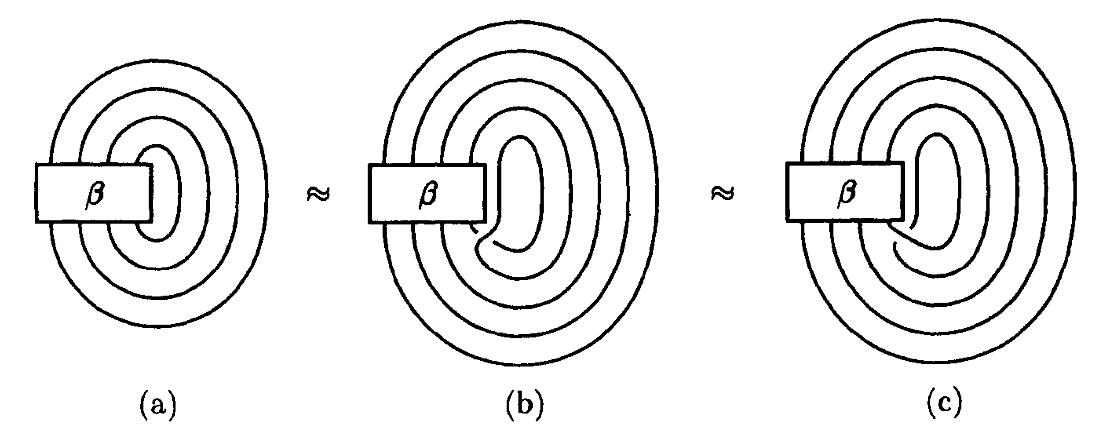
\includegraphics[width=13cm]{Images/movimentos_de_markov.png}
		\end{center}\caption{Movimentos de Markov}
		\label{movimentos de Markov}
	\end{figure}
	%
	É claro que há outras maneiras de obter tranças cujos fechos representam o mesmo \textit{link}, 
	mas, como veremos adiante, as duas transformações acima mostradas nas 
	Figuras \ref{conjugacao nao altera link} e \ref{movimentos de Markov} são especiais. 
	Como foi Markov quem primeiro as introduziu, elas são usualmente chamadas de 
	\textit{movimento de Markov tipo I} e \textit{movimentos de Markov tipo II}. 
	Vamos defini-los formalmente.
	%
	\begin{definition}
		\label{def movimento de Markov tipo 1}
		Um movimento de Markov tipo I, denotado $M_1$, substitui uma trança $\beta$ de $n$ 
		cordas pelo seu conjugado $\gamma\beta\gamma^{-1}$, sendo $\gamma$ uma trança de $n$ 
		cordas arbitrária.  
	\end{definition}
	%
	\begin{definition}
		\label{def movimento de Markov tipo 2}
		Um movimento de Markov do tipo II, denotado $M_2$, substitui a trança $\beta$ 
		de $n$ cordas pela trança $\beta\sigma_n$ ou $\beta\sigma_n^{-1}$ de $n+1$ cordas, 
		sendo $\beta$ visualizada com uma trança de $B_{n+1}(\mathbb{R}^2)$ e $\sigma_n$ 
		um gerador de $B_{n+1}(\mathbb{R}^2)$. 
	\end{definition}
	%
	É claro que podemos definir também os inversos de $M_1$ e $M_2$, que denotaremos por 
	$M_1^{-1}$ e $M_2^{-1}$, respectivamente. Agora, estamos prontos para enunciar o 
	teorema (que não será demonstrado).
	%
	\begin{theorem}[Markov]
		\label{teorema de Markov}
		Suponha $\beta$ e $\beta'$ duas tranças (orientadas) não necessariamente com o mesmo 
		número de cordas. Então, os fechos de $\beta$ e $\beta'$ representam o mesmo 
		\textit{link} ou nó $K$ (orientado) se, e somente se, $\beta$ pode ser deformada 
		em $\beta'$ por uma sequência finita dos movimentos $M_1^{\pm1}, M_2^{\pm1}$. 
		Em símbolos, existe a seguinte sequência finita,
		%
		\begin{align*}
		    \beta = \beta_0\to\beta_1\to\cdots\to\beta_m = \beta'
		\end{align*}
		%
		tal que, para $i = 0,1,\dots,m-1$, $\beta_{i+1}$ é obtida a partir de $\beta_i$ 
		pela aplicação de um dos movimentos $M_1^{\pm1}$ e $M_2^{\pm1}$.
	\end{theorem}
	%
	Podemos, ainda, pensar nos movimentos de Markov para as tranças como paralelos diretos 
	dos movimentos de Reidemeister para \textit{links}. Por conveniência, diremos que 
	duas tranças $\beta$ e $\beta'$ são \textit{Markov equivalentes}, denotado por
	$\beta\underset{M}{\sim}\beta'$, se uma pode ser deformada na outra por meio de uma 
	sequência finita de movimentos de Markov. De fato,
	%
	\begin{prop}
	\label{Markov equivalencia}
		Markov equivalência é uma relação de equivalência.
	\end{prop} 
	%
	\begin{proof}
		Sejam $\alpha$, $\beta$ e $\gamma$ tranças quaisquer, não necessariamente com o 
		mesmo número de cordas. Note que 
		%
		\begin{align*}
		    \alpha = \alpha_0\overset{M_1}{\to}\alpha_1\overset{M_1^{-1}}{\to}\alpha_2 = \alpha,
		\end{align*}
		%
		logo $\alpha\underset{M}{\sim}\alpha$ e, portanto, a relação $\underset{M}{\sim}$ 
		é reflexiva.
		
		\par\vspace{0.3cm} Agora, suponha que $\alpha\underset{M}{\sim}\beta$. Então, por 
		definição, existe uma sequência finita
		%
		\begin{align*}
		    \alpha\to\cdots\to\beta 
		\end{align*}
		%
		de movimentos de Markov que nos permite deformar $\alpha$ em $\beta$. 
		Consequentemente, podemos partir de $\beta$ e, usando a mesma sequência, 
		só que de trás para frente, chegar em $\alpha$. Portanto, $\alpha\underset{M}{\sim}\beta$ 
		implica $\beta\underset{M}{\sim}\alpha$ e a relação $\underset{M}{\sim}$ é simétrica.
		
		\par\vspace{0.3cm} Por fim, suponha $\alpha\underset{M}{\sim}\beta$ e $\beta\underset{M}{\sim}\gamma$. 
		Por definição, existem duas sequências finitas, $S_1$ e $S_2$, digamos, 
		%
		\begin{align*}
    		\alpha\overset{S_1}{\to}\beta, \qquad \beta\overset{S_2}{\to}\gamma
		\end{align*}
		%
		e, consequentemente, existe uma sequência finita $S_3$ de $\alpha$ em $\gamma$
		%
		\begin{align*}
		    \alpha\overset{S_1}{\to}\beta\overset{S_2}{\to}\gamma 
		\end{align*}
		%
		sendo $S_3$ a sequência $S_1$ seguida de $S_2$. Portanto, $\underset{M}{\sim}$ é 
		transitiva e configura uma relação de equivalência.
	\end{proof}
	%
	Com a noção de Markov equivalência, podemos reescrever o Teorema \ref{teorema de Markov} da seguinte forma.
	%
	\begin{theorem}[Markov simplificado]
	\label{teorema de Markov simplificado}
		Sejam $\widetilde{\beta}$ e $\widetilde{\beta'}$ dois \textit{links} (ou nós). 
		Então, $\widetilde{\beta}$ é equivalente a $\widetilde{\beta'}$ se, e somente se,
		$\beta\underset{M}{\sim}\beta'$.
	\end{theorem}
	%
	Algumas observações são necessárias.
	\begin{remark}
		Primeiro, note que o Teorema \ref{teorema de Markov}, em si, não é suficiente para 
		classificarmos todos os \textit{links} e nós. O obstáculo é que, atualmente, não 
		existe nenhum algoritmo conhecido para determinar se duas tranças $\beta$ e $\beta'$ 
		são Markov equivalentes ou não. Dito isso, nos casos relativamente simples de tranças 
		de 2 ou 3 cordas, se os fechos de $\beta$ e $\beta'$ são equivalentes, então 
		(a menos de uma família de tranças de 3 cordas que já foi completamente classificada, 
		vide \cite{classificacao}) 
		$\beta$ e $\beta'$ são conjugadas.
		
		\par\vspace{0.3cm} Segundo, tenha em mente que nos restringimos a \textit{links} e 
		nós \textbf{orientados}. Se ignorarmos a orientação, o teorema de Markov pode não valer. 
		Por exemplo, considere a figura abaixo.
		%
		\begin{figure}[H]
			\begin{center}
				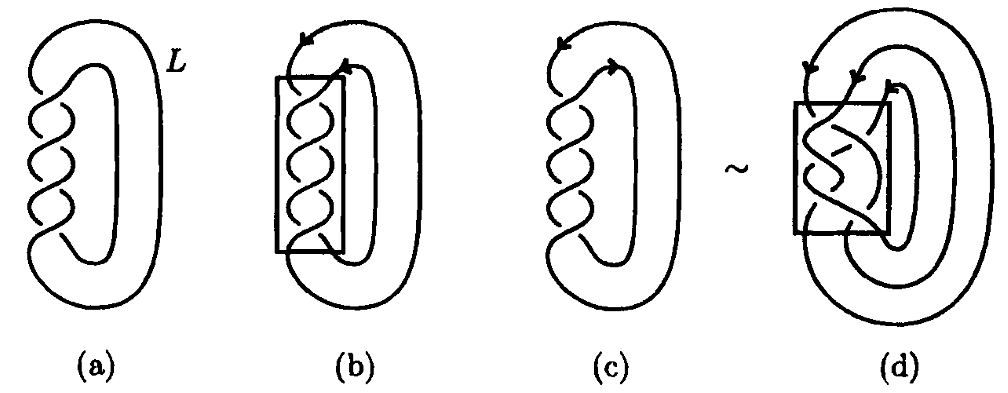
\includegraphics[width=12cm]{Images/orientacao_markov_link.png}
			\end{center}\caption{O \textit{link} $L$ e duas orientações possíveis.}\label{orientacao markov link}
		\end{figure}
		%
		Se orientarmos $L$ como na Figura \ref{orientacao markov link}(b), então 
		(o \textit{link} orientado) $L$ é o fecho da trança de 2 cordas $\sigma_1^4$. 
		Por outro lado, se orientarmos $L$ como na Figura \ref{orientacao markov link}(c), 
		então o mesmo \textit{link} $L$ não pode ser o fecho de nenhuma trança de 2 cordas. 
		Mas, de fato, é possível mostrar que com essa orientação, $L$ na verdade é o fecho 
		da trança de 3 cordas $\sigma_1^{-1}\sigma_2\sigma_1^{2}\sigma_2^{1}$, 
		Figura \ref{orientacao markov link}(d).
		
		\par\vspace{0.3cm} Portanto, o \textit{link} (não orientado) $L$ da 
		Figura \ref{orientacao markov link}(a) pode ser representado por duas tranças distintas, 
		$\sigma_1^4$ e $\sigma_1^{-1}\sigma_2\sigma_1^{2}\sigma_2^{1}$. Contudo, essas duas 
		tranças \textbf{não} são Markov equivalentes.
		
		\par\vspace{0.3cm} Outro exemplo é o da Figura \ref{orientacao markov no}.
		%
		\begin{figure}[H]
			\begin{center}
				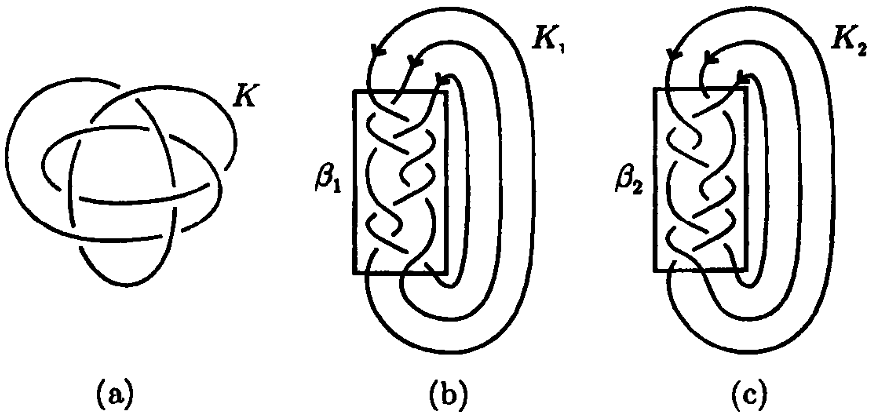
\includegraphics[width=9cm]{Images/orientacao_markov_no.png}
			\end{center}\caption{O nó $K$ e duas orientações possíveis.}\label{orientacao markov no}
		\end{figure}
		%
		É sabido, mas não é fácil mostrar, que os nós (orientados) $K_1$ e $K_2$ da 
		Figura \ref{orientacao markov no}, apesar de obtidos a partir do mesmo nó não 
		orientado $K$, não são equivalentes, justamente por serem dados por orientações 
		diferentes. Pela figura, $K_1$ e $K_2$ são representados pelas tranças $\beta_1$ e $\beta_2$,
		respectivamente. Como $K_1$ e $K_2$ não são equivalentes, então $\beta_1$ e $\beta_2$ 
		não são Markov equivalentes.  
	\end{remark}
	%
	\section{Algumas aplicações do Teorema de Markov}
	\hspace{12pt} Seja $K$ um nó (ou \textit{link}) orientado em $\mathbb{R}^3$. Se considerarmos o plano $xy$ como um espelho, então a imagem de $K$ nesse espelho também é um nó em $\mathbb{R}^3$, veja a figura abaixo.
	
	\begin{figure}[H]
		\begin{center}
			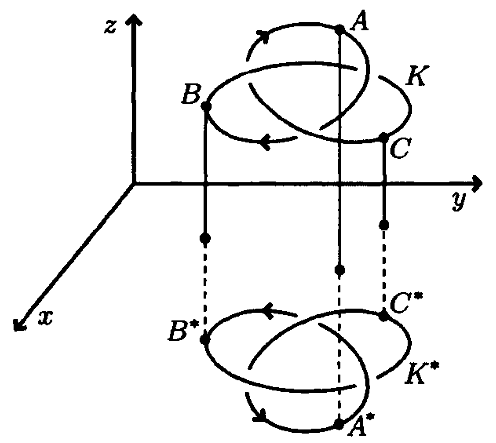
\includegraphics[width=6cm]{Images/no_espelhado.png}
		\end{center}\caption{O nó $K$ refletido em torno do plano $xy$.}\label{no espelhado}
	\end{figure}
	\par\vspace{0.3cm} O nó $K^\ast$ é chamado de imagem espelhada de $K$. Como $K$ é orientado, $K^\ast$ herda uma orientação de $K$.
	\begin{prop}
		\label{troca de cruzamentos}
		Seja $D$ um diagrama (orientado) de um nó $K$. Então, o diagrama $D^\ast$ do nó $K^\ast$ é obtido de $D$ substituindo cruzamentos superiores por cruzamentos inferiores.	
	\end{prop}
	\begin{proof}
		Como a imagem espelhada de $K$ é obtida a partir de uma rotação de $K$, então os cruzamentos superiores passam a ser inferiores e vice-versa.
	\end{proof}
	\par\vspace{0.3cm} Na Figura \eqref{no de trevo} abaixo estão representados os diagramas $D$ e $D^\ast$ de um nó $K$. Esse nó $K$ é chamado de \textit{nó de trevo}.
	
	\begin{figure}[H]
		\begin{center}
			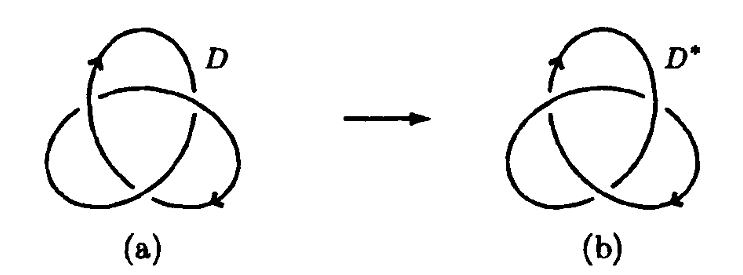
\includegraphics[width=9cm]{Images/no_de_trevo.png}
		\end{center}\caption{O nó de trevo orientado.}
		\label{no de trevo}
	\end{figure} 
	
	\par\vspace{0.3cm} Apesar de que, em geral, um nó e sua imagem espelhada não são equivalentes, há casos em que isso acontece. Um nó que é equivalente a sua imagem espelhada é chamado de \textit{anfiquiral} ou \textit{aquiral}. Um exemplo de nó aquiral é o nó da figura abaixo.
	
	\begin{figure}[H]
		\begin{center}
			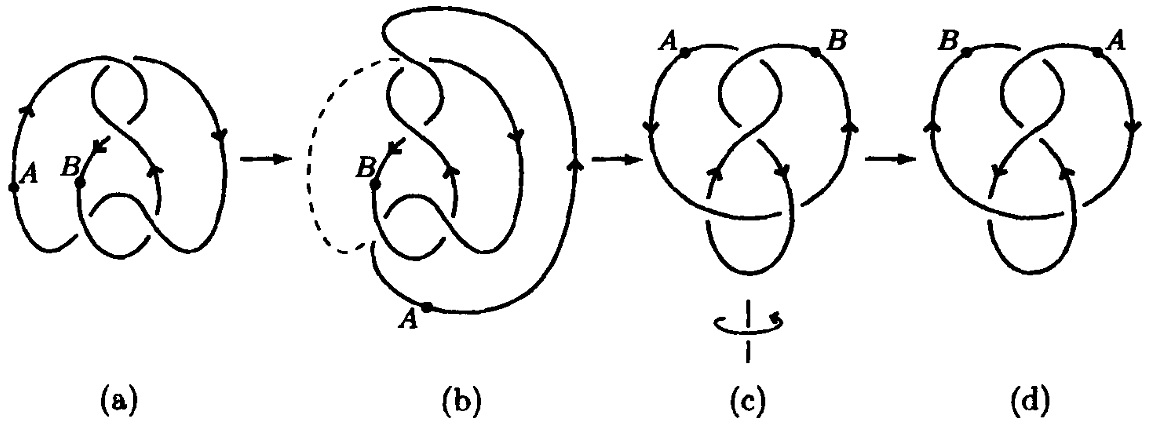
\includegraphics[width=11cm]{Images/no_aquiral.png}
		\end{center}\caption{O nó figura oito, um exemplo de nó aquiral.}\label{no aquiral}
	\end{figure}
	
	\par\vspace{0.3cm} O nó da Figura \eqref{no aquiral}(a), representado pelo diagrama $D$, pode ser representado pelo fecho da trança de $3$ cordas $\beta = \sigma_1\sigma_2^{-1}\sigma_1\sigma_2^{-1} = (\sigma_1\sigma_2^{-1})^2$. Na sua forma de trança, a imagem espelhada $K^\ast$ de $K$ é exatamente o fecho da trança $\beta^{-1}$ (com a orientação inversa), como mostra a figura abaixo.
	
	\begin{figure}[H]
		\begin{center}
			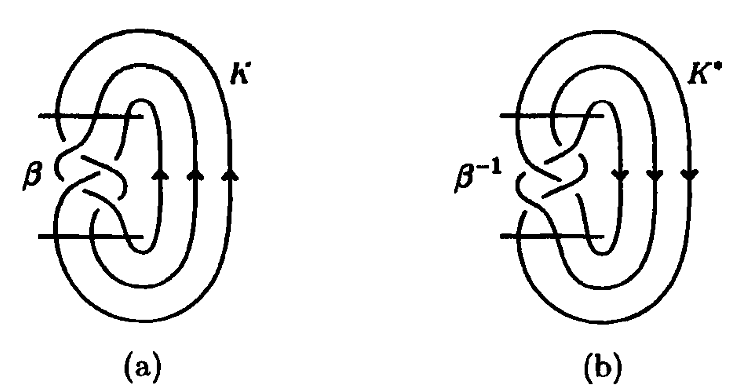
\includegraphics[width=10cm]{Images/tranca_no_de_oito.png}
		\end{center}\caption{Trança do nó figura oito.}\label{tranca no de oito}
	\end{figure} 
	
	\par\vspace{0.3cm} Esse exemplo suscita a pergunta: dado um nó (ou \textit{link}) orientado e uma trança que representa esse nó, como podemos expressar $K^\ast$ baseados em $\beta$? A resposta está na proposição a seguir.
	
	\begin{prop}
		\label{representacao no espelhado}
		Seja $K$ um nó (ou \textit{link}) orientado e suponha que $K$ é o fecho de uma trança de $n$ cordas $\beta = \sigma_{i_1}^{\varepsilon_1}\cdots\sigma_{i_k}^{\varepsilon_k}$, sendo $1\leq i_1, i_2, \dots, i_k\leq n-1$ e $\varepsilon_i=\pm1$. Então, 
		\begin{enumerate}
			\item a imagem espelhada $K^\ast$ de $K$, com a orientação invertida, pode ser representada como o fecho de 
			$\beta^{-1}  = \sigma_{i_k}^{-\varepsilon_{k}}\cdots\sigma_{i_1}^{-\varepsilon_1}$ 
			\item o nó $\overline{K}$ obtido de $K$ revertendo a orientação de $K$ pode ser representado por
			
			\begin{align*}
			\overline{\beta} = \sigma_{i_k}^{\varepsilon_k}&\cdots\sigma_{i_i}^{\varepsilon_1} \\
			&\text{ou} \\
			\overline{\overline{\beta}} = \sigma_{n-i_k}^{\varepsilon_k}&\cdots\sigma_{n - i_1}^{\varepsilon_1}
			\end{align*}
			\par\vspace{0.3cm} e, portanto, $\overline{\beta}\underset{M}{\sim}\overline{\overline{\beta}}$. 
		\end{enumerate}
	\end{prop}
	
	\begin{proof}
		A demonstração do item 1 segue diretamente dos diagramas da Figura \eqref{tranca no de oito}. De fato, inverter a orientação de $K$ equivale a espelhar a trança $\beta$, ou seja, invertê-la. Para o item 2, observe a Figura \eqref{no invertido}, que ilustra o processo aqui descrito. Primeiro, mude a orientação da Figura \eqref{no invertido}(a) para obter a Figura \eqref{no invertido}(b). Então, vire a Figura \eqref{no invertido}(b) de cabeça para baixo, Figura \eqref{no invertido}(c). Em seguida, rotacione a Figura \eqref{no invertido}(c) em torno do eixo vertical por um ângulo de $\pi$ radianos, Figura \eqref{no invertido}(d). Podemos ver que a Figura \eqref{no invertido}(c) é $\overline{\overline{\beta}}$ e que a Figura \eqref{no invertido}(d) é $\overline{\beta}$. Como não alteramos o nosso nó $\overline{K}$, então os fechos de $\overline{\beta}$ e $\overline{\overline{\beta}}$ são equivalentes e representam o mesmo nó, $\overline{K}$. Por fim, pelo Teorema \eqref{teorema de Markov simplificado}, temos $\overline{\beta}\underset{M}{\sim}\overline{\overline{\beta}}$.
		
		\begin{figure}[H]
			\begin{center}
				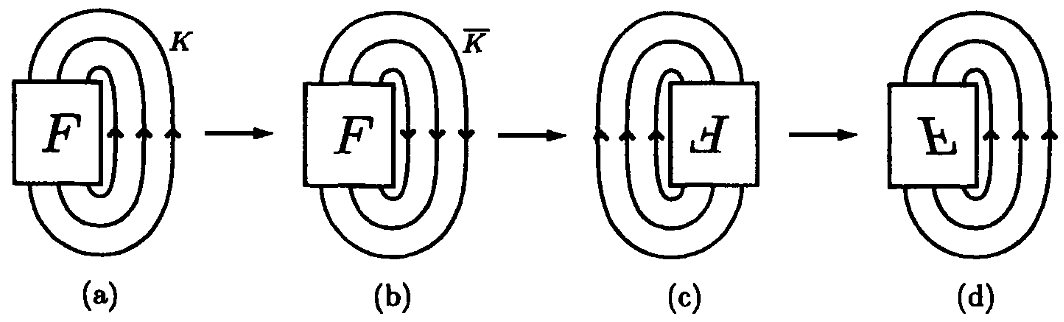
\includegraphics[width=12cm]{Images/no_invertido.png}
			\end{center}\caption{Inversão da orientação de um nó.}\label{no invertido}
		\end{figure}
		
		\par\vspace{0.3cm} 
		
	\end{proof}
	\par\vspace{0.3cm} Se os nós $K$ e $\overline{K}$ são equivalentes, então $K$ é dito \textit{inversível}. O nó da Figura \eqref{no aquiral}(a) é inversível, uma vez que os dois nós das Figuras \eqref{no aquiral}(c) e (d) são equivalentes. Apesar de muitos nós serem inversíveis, isso não quer dizer que todos os nós o são. De fato, um contraexemplo é o nó $K$ da Figura \eqref{orientacao markov no}.
	%COMECEI AQUI
	\section{Grupos de nó}
	\hspace{12pt} Até agora, tratamos de nós de maneira um tanto quanto informal. Contudo, assim como fizemos para a trança, podemos tomar uma abordagem mais topológica. De fato, podemos utilizar, assim como foi com as tranças, grupos fundamentais. Para isso, recorde que definimos nó como uma curva poligonal simples fechada em $\mathbb{R}^3$. Contudo, por conveniência, é comum substituir $\mathbb{R}^3$ por $\mathbb{S}^3$ (a 3-esfera unitária), pois $\mathbb{S}^3$ pode ser obtida de $\mathbb{R}^3$ adicionando um único ponto (de fato, isso é verdade para $\mathbb{S}^n$ e $\mathbb{R}^n$, realizando-se um análogo da projeção estereográfica para dimensões superiores. Como exercício, imagine o caso $n = 1$. Informalmente, estamos adicionando a $\mathbb{R}$ o ``ponto infinito'', $\infty$.)
	\par\vspace{0.3cm} Nesse contexto, podemos definir o \textit{complemento de um nó}.
	\begin{deff}
		\label{def complemento no}
		Dado um nó $K$, o complemento de $K$ é o subconjunto $\mathbb{S}^3 - K$ de $\mathbb{S}^3$.
	\end{deff}
	\par\vspace{0.3cm} Com essa definição, podemos então definir o \textbf{grupo fundamental do complemento de nó}, muitas vezes chamado simplesmente de \textbf{grupo fundamental de nó}.
	\begin{deff}
		\label{grupo fundamental de no}
		O grupo fundamental de um nó $K$ com ponto base $b\in\mathbb{S}^3 - \text{Im}(K)$ é o grupo fundamental do complemento de $K$, com $b$ como ponto base.
	\end{deff}
	\par\vspace{0.3cm} Como $\mathbb{S}^3$ é conexo por caminhos, podemos omitir o ponto base, pois a escolha dele não afeta a estrutura de grupo. Em síbolos, denotamos o grupo fundamental do nó $K$ por $\pi_1(\mathbb{S}^3\setminus K)$. 
	\par\vspace{0.3cm} Um primeiro exemplo é o grupo fundamental do nó trivial. Apesar do nó ser trivial, seu grupo não o é; de fato, o grupo fundamental do nó trivial é o grupo cíclico infinito, $\mathbb{Z}$. Outro exemplo é o nó de trevo, mostrado na figura \eqref{no de trevo}; o seu grupo fundamental tem apresentação 
	\begin{align*}
	\langle x,y|x^3 = y^2 \rangle
	\end{align*}
	\par\vspace{0.3cm} ou seja, o grupo do nó de trevo é (isomorfo a) $B_3(\mathbb{R}^2)$! Um último exemplo é o nó figura oito, mostrado na figura \eqref{no aquiral}; seu grupo fundamental tem apresentação
	\begin{align*}
	\langle x,y | yxy^{-1}xy = xyx^{-1}yx \rangle
	\end{align*}
	\par\vspace{0.3cm} O grupo fundamental de nó também é um invariante: se dois nós são equivalentes, então seus grupos fundamentais são isomorfos. Contudo, o contrário não é verdadeiro. Por exemplo, os dois nós de trevo abaixo têm o mesmo grupo fundamental, mas não são equivalentes (pois o nó de trevo é quiral, como vimos).
	
	\begin{figure}[H]
		\begin{center}
			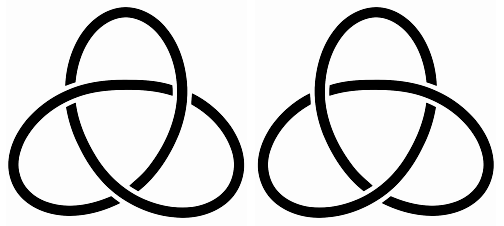
\includegraphics[width=6cm]{Images/nos_de_trevo.png}
		\end{center}\caption{Os nós de trevo destro (à esquerda) e canhoto (à direita).}\label{nos de trevo destro e canhoto}
	\end{figure} 
	
	\par\vspace{0.3cm} Uma das maiores questões quando estudamos nós é determinar se dois nós são ou não equivalentes, ou seja, como podemos distinguir dois nós. Uma das ferramentas que nos ajuda nessa tarefa são os chamados \textit{invariantes de nós}. Demos um exemplo de invariante de nó acima, a saber, o número de componentes $\mu(\beta)$. Esse invariante era, de certo modo, esperado, uma vez que não podemos ``cortar'' nosso nó, ou seja, é impossível alterar o número de componentes por meio de movimentos de Reidemeister ($\Omega_1^{\pm1}$, $\Omega_2^{\pm1}$ e $\Omega_3^{\pm1}$). Outros exemplos de invariantes são o polinômio de Alexander e o polinômio de Jones, que serão abordados a seguir. Antes, porém, uma curiosidade.
	\par\vspace{0.3cm} Um tipo particular de nó são os chamados \textit{nós de toro} (ou \textit{nós torais}). Como o nome sugere, são nós que pertencem à superfície de um toro (que, por sua vez, é um subconjunto de $\mathbb{R}^3$). Podemos definir um nó de toro usando coordenadas da seguinte forma.\footnote{Veja \cite{no-toral}.}
	
	\begin{deff}
		\label{def no de toro}
		Para todo par de inteiros $a$ e $b$ coprimos, o nó de toro padrão $K_{a,b}: \mathbb{S}^1\to\mathbb{S}^3$ correspondente ao par $(a,b)$ é dado, em coordenadas Euclidianas, por 
		\begin{align*}
		\theta\mapsto
		\left( 
		\begin{matrix}
		(2+\cos(b\theta))\cos(a\theta) \\
		(2+\cos(b\theta))\sin(a\theta) \\
		-\sin(a\theta)
		\end{matrix} 
		\right)
		\end{align*}	
	\end{deff}
	\par\vspace{0.3cm} Essa função é uma imersão do círculo ($\mathbb{S}^1$) no toro $T$ parametrizado por
	\begin{align*}
	(\theta, \varphi)\mapsto 
	\left( \begin{matrix}
	(2+\cos(\theta))\cos(\varphi) \\
	(2+\cos(\theta))\sin(\varphi) \\
	\sin(\theta)
	\end{matrix}  \right)
	\end{align*}
	\begin{figure}[H]
		\begin{center}
			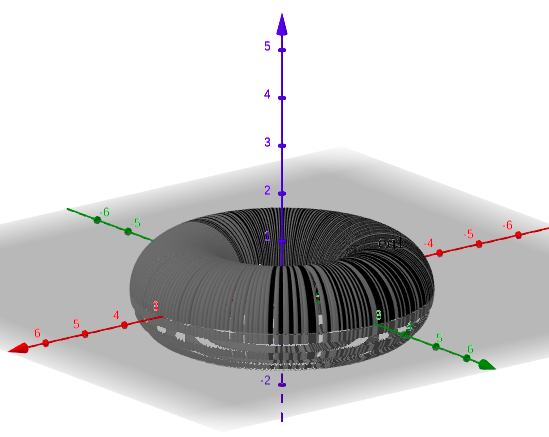
\includegraphics[width=8cm]{Images/toro.png}
		\end{center}\caption{O toro $T$ em $\mathbb{R}^3$.}\label{toro}
	\end{figure}
	\par\vspace{0.3cm} Os exemplos mais simples de nós torais são os nós de toro $K_{2,3}$ e $K_{2,-3}$, que são os nós de trevo destro e canhoto, respectivamente. Note que os nós de trevo ficam completamente contidos na superfície do toro $T$, assim como todos os nós torais. Em particular, se $a = \pm1$ ou se $b = \pm1$, então o nó $K_{a,b}$ resultante é trivial.
	
% 	\begin{figure}[H]
% 		\centering
% 		\begin{subfigure}[t]{0.5\textwidth}
% 			\centering
% 			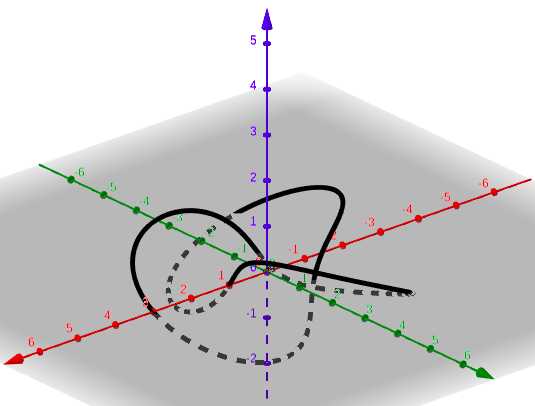
\includegraphics[width=6cm,height=5cm]{Images/no_de_trevo_parametrizado.png}
% 			\caption{}
% 		\end{subfigure}%
% 		~ 
% 		\begin{subfigure}[t]{0.5\textwidth}
% 			\centering
% 			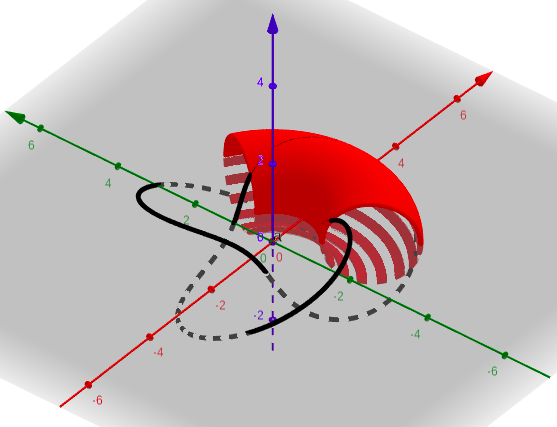
\includegraphics[width=6cm,height=5cm]{Images/no_de_trevo_no_toro.png}
% 			\caption{}
% 		\end{subfigure}
% 		\caption{O nó toral $K_{2,3}$ (nó de trevo destro), figura (a) e parte do toro, envolvendo $K_{2,3}$, figura (b)}
% 	\end{figure}
	
	\begin{figure}[H]
        \centering
        \subfloat[]{{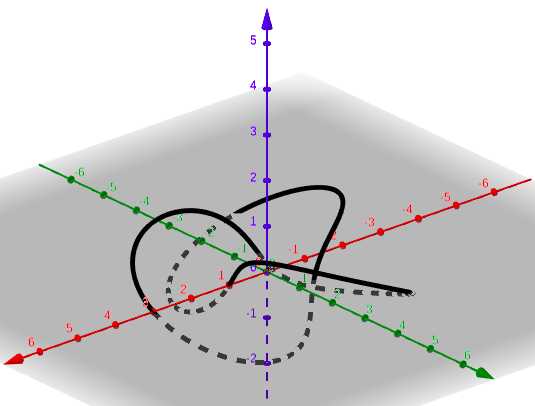
\includegraphics[width=6cm,height=5cm]{Images/no_de_trevo_parametrizado.png}}}\hfill
        \subfloat[]{{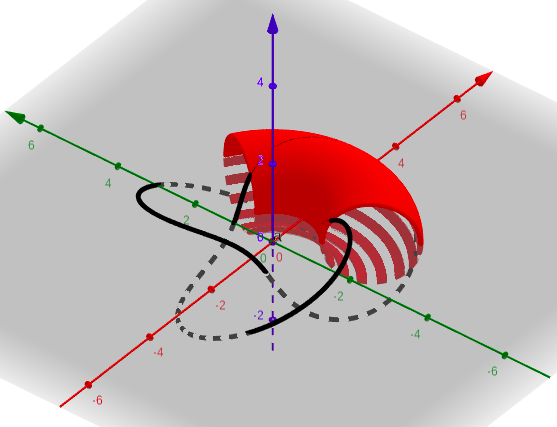
\includegraphics[width=6cm,height=5cm]{Images/no_de_trevo_no_toro.png}}}
        \caption{O nó toral $K_{2,3}$ (nó de trevo destro), figura (a) e parte do toro, envolvendo $K_{2,3}$, figura (b)}
    \end{figure}
	
	%\newpage
	\par\vspace{0.3cm} É interessante observar que, sem a restrição de $(a,b)$ coprimos, a função de $K_{a,b}:\mathbb{S}^1\to\mathbb{S}^3$ descreve um \textit{link}. Logo, podemos generalizar a Definição \eqref{def no de toro} para \textit{links}, da seguinte forma.
	\begin{deff}
		\label{def link de toro}
		Para todo par de inteiros $a$ e $b$ (não necessariamente coprimos), o \textit{link} de toro (ou link toral) padrão $K_{a,b}: \mathbb{S}^1\to\mathbb{S}^3$ correspondente ao par $(a,b)$ é dado, em coordenadas Euclidianas, por 
		\begin{align*}
		\theta\mapsto
		\left( 
		\begin{matrix}
		(2+\cos(b\theta))\cos(a\theta) \\
		(2+\cos(b\theta))\sin(a\theta) \\
		-\sin(a\theta)
		\end{matrix} 
		\right)
		\end{align*}
		\par\vspace{0.3cm} O número de componentes do link correspondente ao par $(a,b)$ é dado por $d = \mdc(a,b)$, e cada componente é uma cópia do nó $\displaystyle{K_{a/d, b/d}}$ rotacionado em torno do eixo $z$.
	\end{deff}
	\par\vspace{0.3cm} Uma propriedade interessante é que todo nó toral não trivial é quiral, i.e., não é igual à sua imagem espelhada (daí a nomenclatura ``destro'' e ``canhoto''). Por fim, vale mencionar que todo nó toral $K_{a,b}$ pode ser representado pela trança fechada $(\sigma_1\sigma_2\cdots\sigma_{a-1})^b$.  
	
	\subsection{Cálculo do grupo de nó}
	\hspace{12pt} Como dito antes, dados dois nós equivalentes $K_1$ e $K_2$, então $\pi_1(\mathbb{R}^3\setminus K_1) \cong \pi_1(\mathbb{R}^3\setminus K_2)$. Contudo, novamente, a recíproca não é verdadeira: $\pi_1(\mathbb{R}^3\setminus K_1) \cong \pi_1(\mathbb{R}^3\setminus K_2)$ não implica $K_1$ e $K_2$ equivalentes. 
	\par\vspace{0.3cm} Se queremos usar os grupos de nó para obter informações acerca dos nós, devemos ser capazes de efetivamente determinar esses grupos. Felizmente, existe um algoritmo simples, introduzido por Wirtinger por volta de 1904 em suas aulas em Vienna e publicado em 1908 por Tietze. Vamos descrever o \textbf{método de Wirtinger}.
	\subsubsection*{Algoritmo de Wirtinger}
	\hspace{12pt} Suponha que temos uma projeção de nó.
	\begin{enumerate}
		\item Fixe uma direção ao longo de $K$ e denote os arcos sucessivos entre dois cruzamentos inferiores por $\alpha_1, \dots, \alpha_n$.
		\item Para $1\leq i\leq n$, desenhe um seta curta $x_i$ passando por baixo de $\alpha_i$, em que a direção de $x_i$ é dada pela regra da mão direita, com o dedão apontando na direção escolhida sobre $K$. Tal seta representa um \textit{loop} em $\mathbb{R}^3\setminus K$ do seguinte modo: tome um ponto base acima do plano de desenho; então o \textit{loop} consiste do triângulo orientado a partir do ponto base para a cauda de $x_i$, ao longo de $x_i$ até a ponta e de volta para o ponto base.
		\begin{figure}[H]
			\begin{center}
				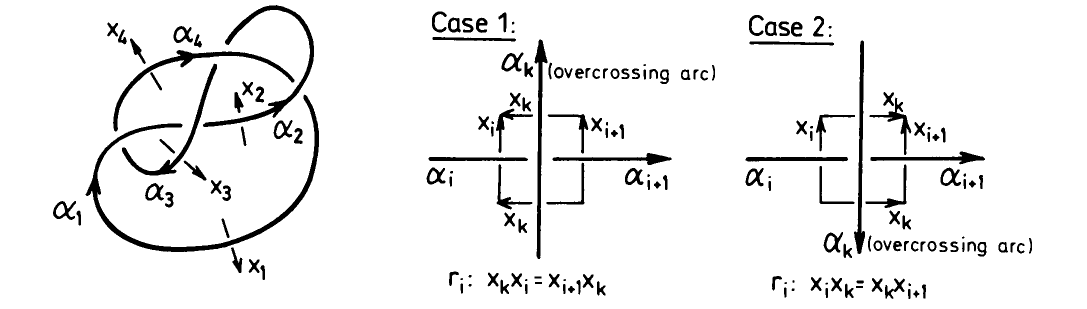
\includegraphics[width=15cm]{Images/arcosgrupono.png}
			\end{center}\caption{Desenhos possíveis}
			\label{desenhos possiveis}
		\end{figure}
		\item Em cada cruzamento, indique o quadrado formado pelas setas sob os arcos envolvidos no cruzamento, e escreva a relação $r_i$ indicada por esse quadrado; há duas possibilidades dadas pelos desenhos na Figura \eqref{desenhos possiveis}(note que $k=i$ ou $k=i+1$ é possível)
		\par Então o grupo do nó $K$ é gerado por (classes de homotopia de) \textit{loops} $x_i$ e tem apresentação
		\begin{align*}
		\tag{Apresentação de Wirtinger}
		\pi_1(\mathbb{R}^3\setminus K) = \left< x_1, \dots, x_n \ | \ r_1, \dots, r_n \right>
		\end{align*}
		\par Ademais, qualquer das relações $r_i$ é consequência das $n-1$ relações restantes e pode, portanto, ser omitida.
	\end{enumerate}
	\par\vspace{0.3cm} Não vamos, aqui, demonstrar precisamente o teorema, mas vamos dar algumas observações. É razoavelmente claro, geometricamente, que $\pi_1(\mathbb{R}^3\setminus K)$ é gerado pelos \textit{loops} $x_i$; para qualquer \textit{loop} em $\mathbb{R}^3\setminus K$, basta checar quantas voltas ele dá em cada um dos arcos $\alpha_i$ e deformá-lo conformemente. Também é claro que as relações $r_i$ devem valer, i.e., que $x_kx_ix_k^{-1}x_{i+1}^{-1}$ (caso 1) ou $x_ix_kx_{i+1}^{-1}x_k^{-1}$ (caso 2) podem ser reduzidas a um ponto em $\mathbb{R}^3\setminus K$. Isso é mostrado nas seguintes figuras.
	\begin{figure}[H]
		\begin{center}
			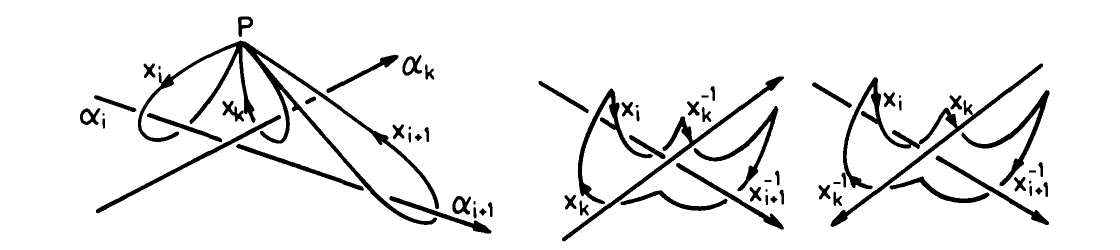
\includegraphics[width=15cm]{Images/deformacaoloops.png}
		\end{center}\caption{Redução em cada caso}
	\end{figure}
	\par\vspace{0.3cm} O que não é tão óbvio é que nenhuma relação adicional vale e que qualquer uma das $n$ relações pode ser omitida. Vamos olhar os dois exemplos dados acima, do nó de trevo e do nó figura oito, mais de perto.
	\begin{example}[Nó de trevo]
		Seja $K$ o nó de trevo dado abaixo.
		\begin{figure}[H]
			\begin{center}
				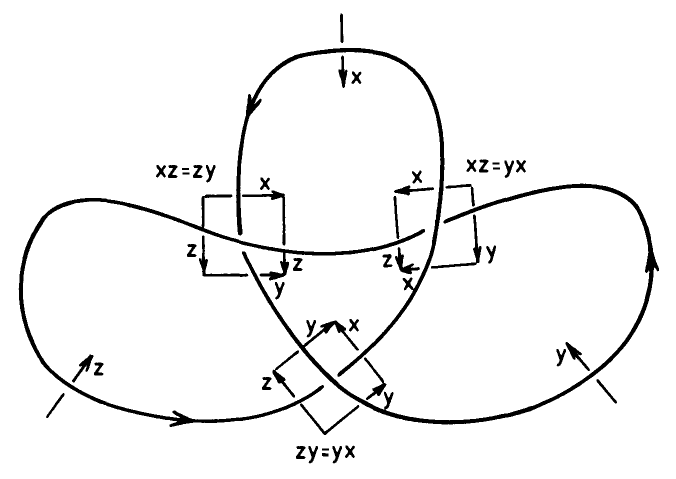
\includegraphics[width=12cm]{Images/gruponotrevo.png}
			\end{center}\caption{Cálculo do grupo de nó do nó de trevo.}
			\label{grupo no de trevo}
		\end{figure}
		\par\vspace{0.3cm} Usando a terminologia da figura, vemos que $\pi_1(\mathbb{R}^3\setminus K)$ é gerado por $3$ elementos $x, y, z$, sujeitos às relações $xz = zy, xz = yx$ e $zy = yx$. De acordo com o teorema de Wirtinger, qualquer uma dessas relações, digamos a terceira, pode ser omitida; isso pode ser verificado algebricamente: eliminando $z = x^{-1}yx$ da segunda relação, a primeira relação se torna $xyx = yxy$. Logo, obtemos uma apresentação para $\pi_1(\mathbb{R}^3\setminus K)$ do nó de trevo:
		\begin{align*}
		\pi_1(\mathbb{R}^3\setminus K) = \left< x,y \ | \ xyx = yxy \right>
		\end{align*}
		\par\vspace{0.3cm} Fazendo $a = xyx$ e $b = xy$, temos $x = b^{-1}a, y = a^{-1}b^2$ e $a^2 = (xyx)^2 = (xyx)(xyx) = (xyx)(yxy) = (xy)^3 = b^3$. Assim, podemos escrever o grupo do nó de trevo como
		\begin{align*}
		\pi_1(\mathbb{R}^3\setminus K) = \left< a,b \ | \ a^2 = b^3 \right>
		\end{align*}
		\par\vspace{0.3cm} Note que $\alpha = (12)$ e $\beta = (123)$ em $S_3$ também satisfazem $\alpha^2 = \beta^3 = e$. Logo, $S_3$ é imagem homomórfica de $\pi_1(\mathbb{R}^3\setminus K)$, o que implica que $\pi_1(\mathbb{R}^3\setminus K)$ não é abeliano. Em particular, o grupo de $K$ não é isomorfo ao grupo do nó trivial ($\mathbb{Z}$), logo $K$ não pode ser desatado sem cortes e colagens (como esperado).
	\end{example}
	\begin{example}[Nó figura oito]
		O nó figura oito é mostrado abaixo.
		\begin{figure}[H]
			\begin{center}
				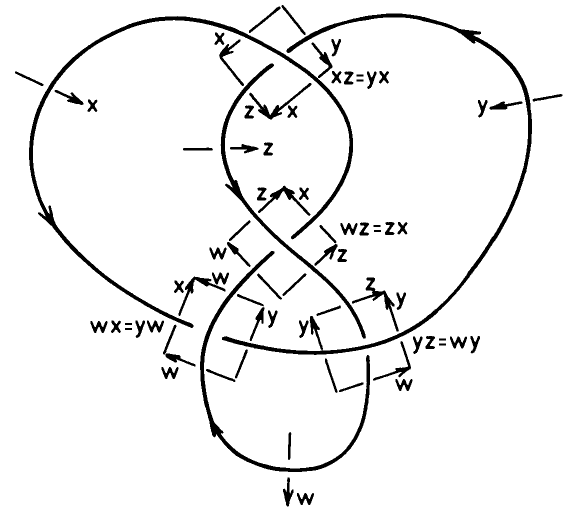
\includegraphics[width=10cm]{Images/gruponooito.png}
			\end{center}\caption{Cálculo do grupo de nó do nó figura oito}
			\label{grupo no de oito}	
		\end{figure}
		\par\vspace{0.3cm} O algoritmo de Wirtinger nos dá quatro geradores $x,y,z,w$ e quatro relações $xz = yx, wz = zx, yz = wy$ e $wx = yw$. Novamente, a última dessas relações pode ser omitida. Escrevemos a primeira relação na forma $z = x^{-1}yx$ e então a segunda relação na forma $w = zxz^{-1} = (x^{-1}yx)x(x^{-1}y^{-1}x) = x^{-1}yxy^{-1}x$; e a última relação, a terceira, torna-se $yx^{-1}yx = x^{-1}yxy^{-1}xy$. Logo, o grupo $\pi_1(\mathbb{R}^3\setminus K)$ do nó de trevo pode ser apresentado como
		\begin{align*}
		\pi_1(\mathbb{R}^3\setminus K) = \left< x,y \ | \ yx^{-1}yx = x^{-1}yxy^{-1}xy \right>
		\end{align*}
	\end{example}
	\par\vspace{0.3cm} Se dois nós têm grupos não isomorfos, então não é possível deformar um dos nós no outro; em particular, se o grupo de um nó não é isomorfo a $\mathbb{Z}$, então esse nó não é trivial. Portanto, podemos utilizar a teoria dos grupos para distinguir tipos diferentes de nós. Contudo, vale pontuar que se dois nós são dados por uma apresentação (como a apresentação de Wirtinger), em geral é um problema algébrico difícil decidir se esses grupos são isomorfos ou não.
	\par\vspace{0.3cm} Por outro lado, pode ser nos dado o problema puramente algébrico de decidir se dois grupos dados por apresentações são isomorfos ou não. Se soubermos que esses grupos ocorrem como grupos de nó, e também soubermos, por considerações topológicas, que esses nós não são equivalentes, então podemos concluir que esses dois grupos não são isomorfos. Portanto, não apenas a teoria dos grupos ajuda a topologia, mas reciprocamente!
	
	\section{Representação de Burau e os polinômios de Alexander e Jones} 
	\hspace{12pt} Como consequência do Teorema \eqref{teorema de Markov}, podemos usar tranças e a teoria das tranças para determinar invariantes de nós. Um dos exemplos mais elegantes desse método é o chamado \textit{polinômio de Alexander}, nomeado em homenagem ao matemático norte-americano J.W. Alexander, e denotado por $\Delta_K(t)$, sendo $K$ um nó (ou \textit{link}).
	\par\vspace{0.3cm} Mesmo com a descoberta do polinômio de Jones (outro invariante que também será tratado mais à frente) e seus híbridos em 1980, o polinômio de Alexander ainda permanece, mesmo após mais de 50 anos de pesquisa, um dos mais importantes e úteis invariantes de nós (e \textit{links}).
	\par\vspace{0.3cm} Para definir o polinômio de Alexander, devemos primeiro introduzir a chamada \textit{representação de Burau} de $B_n(\mathbb{R}^2)$. Então, seja $\beta\in B_n(\mathbb{R}^2)$. Podemos representar essa trança como
	\begin{align*}
	\beta = \sigma_{i_1}^{\varepsilon_1}\cdots\sigma_{i_k}^{\varepsilon_k}
	\end{align*}
	\par\vspace{0.3cm} com $1\leq i_1, \dots, i_k\leq n-1$ e $\varepsilon_i = \pm1$. Agora, vamos definir a função
	\begin{align*}
	\varphi_n: B_n\to M(n, \mathbb{Z}[t, t^{-1}])
	\end{align*}
	sendo $M(n, \mathbb{Z}[t,t^{-1}])$ as matrizes de ordem $n$ sobre o módulo $\mathbb{Z}[t,t^{-1}]$, tal que
	\begin{equation}
	\label{representacao de Burau}
	\varphi_n(\sigma_i) = 
	\left[ 
	\begin{array}{c|cc|c}
	I_{i-1} &  &  & \\
	\hline 
	& 1-t & t &  \\
	& 1 & 0 &  \\ 
	\hline
	&  &  & I_{n-i-1}
	\end{array}
	\right] 
	\end{equation}
	\par\vspace{0.3cm} sendo $I_m$ a matriz identidade de ordem $m$ e os espaços vazios correspondem a matrizes nulas. A representação de $B_n$ dada em \eqref{representacao de Burau} é chamada \textit{representação de Burau}. De fato, $\varphi_n$ é homomorfismo, como mostraremos a seguir.
	\begin{prop}
		\label{Burau e homomorfismo}
		A função $\varphi_n$ definida em \eqref{representacao de Burau} é homomorfismo. 
	\end{prop}
	\begin{proof}
		Basta mostrarmos que toda relação de $B_n$ é mapeada na matriz identidade ou, equivalentemente, que as relações de $B_n$ se mantêm para $\varphi_n$. 
		\par\vspace{0.3cm} Primeiro, vamos mostrar que se $|i - j|\geq 2$, então $\varphi_n(\sigma_i)\varphi_n(\sigma_j) = \varphi_n(\sigma_j)\varphi_n(\sigma_i)$. Sem perda de generalidade, podemos tomar $j>i+1$ e, portanto
		\begin{equation*}
		\varphi_n(\sigma_i)\varphi_n(\sigma_j) = 
		\left[ 
		\begin{array}{c|cc|c|cc|c}
		I_{i-1} & & & & & & \\
		\hline
		& 1-t & t & & & & \\
		& 1 & 0 & & & & \\
		\hline
		& & & I_{j-i-2} & & &\\
		\hline
		& & & & 1-t & t &\\
		& & & & 1 & 0 & \\
		\hline 
		& & & & & & I_{n-j-1} 
		\end{array}	
		\right] = \varphi_n(\sigma_j)\varphi_n(\sigma_i)
		\end{equation*}
		\par\vspace{0.3cm} sendo os espaços vazios preenchidos por matrizes nulas.
		\par\vspace{0.3cm} Agora, para a segunda e última relação, $\sigma_i\sigma_{i+1}\sigma_i = \sigma_{i+1}\sigma_i\sigma_{i+1}$, basta considerarmos o caso $n=3$, uma vez que na representação de Burau as entradas não nulas correspondem a matrizes identidade, ou seja, aumentando $n$ a partir de $3$, estaremos apenas acrescentando uma nova linha e uma nova coluna que serão ambas nulas com exceção da entrada diagonal, que será $1$; portanto, a multiplicação das matrizes não é afetada. 
		\par\vspace{0.3cm} Então, tomando $n = 3$, temos
		\begin{align*}
		\varphi_3(\sigma_1\sigma_2\sigma_1) &= \varphi_3(\sigma_1)\varphi_3(\sigma_2)\varphi_3(\sigma_1) \\ &= 
		\begin{bmatrix}
		1-t & t & 0 \\
		1 & 0 & 0 \\
		0 & 0 & 1
		\end{bmatrix}\begin{bmatrix}
		1 & 0 & 0 \\
		0 & 1-t & t \\
		0 & 1 & 0
		\end{bmatrix}\begin{bmatrix}
		1-t & t & 0 \\
		1 & 0 & 0 \\
		0 & 0 & 1
		\end{bmatrix} \\
		&= \begin{bmatrix}
		(1-t)^2 +t(1-t) & t(1-t) & t^2 \\
		1-t & t & 0 \\
		1 & 0 & 0
		\end{bmatrix} \\
		&= \begin{bmatrix}
		1 & 0 & 0 \\
		0 & 1-t & t \\
		0 & 1 & 0
		\end{bmatrix}\begin{bmatrix}
		1-t & t & 0 \\
		1 & 0 & 0 \\
		0 & 0 & 1
		\end{bmatrix}\begin{bmatrix}
		1 & 0 & 0 \\
		0 & 1-t & t \\
		0 & 1 & 0
		\end{bmatrix}\\
		&= \varphi_3(\sigma_2)\varphi_3(\sigma_1)\varphi_3(\sigma_2)\\
		&=\varphi_3(\sigma_2\sigma_1\sigma_2)
		\end{align*}
	\end{proof}
	\begin{remark}
		Em geral, a função $\varphi_n$ não é fiel, i.e., injetiva. Para $n=2$ e $n=3$, é sabido que $\varphi_n$ é fiel; para $n=4$, contudo, não sabemos.
	\end{remark}
	\par\vspace{0.3cm} Note também que como $\det(\varphi_n(\sigma_i)) = -t$ (basta expandir o determinante pelas primeiras $i-1$ linhas e, em seguida, pelas últimas $n-i-1$ linhas, restando apenas a matriz $\left[\begin{smallmatrix}
	1-t & t \\
	1 & 0
	\end{smallmatrix}\right]$), então existe o inverso de $\varphi_n(\sigma_i)$. Para computá-lo, note que
	\begin{align*}
	\varphi_n(1) = I_n = \varphi_n(\sigma_i\sigma_i^{-1}) = \varphi_n(\sigma_i)\varphi_n(\sigma_i^{-1}) \Leftrightarrow \varphi_n(\sigma_i^{-1}) = (\varphi_n(\sigma_i))^{-1}
	\end{align*} 
	\par\vspace{0.3cm} Calculando o inverso de $\varphi_n(\sigma_i)$ (que se resume basicamente a encontrar o inverso de $\left[\begin{smallmatrix}
	1-t & t\\
	1 & 0
	\end{smallmatrix}\right]$), obtemos
	\begin{align*}
	\varphi_n(\sigma_i^{-1}) = 
	\left[ 
	\begin{array}{c|cc|c}
	I_{i-1} &  &  & \\
	\hline 
	& 0 & 1 &  \\
	& t^{-1} & 1-t^{-1} &  \\ 
	\hline
	&  &  & I_{n-i-1}
	\end{array}
	\right] 
	\end{align*}
	\par\vspace{0.3cm} Por exemplo, tomando $\beta = \sigma_1\sigma_2^{-1}$, temos
	\begin{align*}
	\varphi_3(\beta) &= 
	\begin{bmatrix}
	1-t & t & 0 \\
	1 & 0 & 0 \\
	0 & 0 & 1
	\end{bmatrix}\begin{bmatrix}
	1 & 0 & 0 \\
	0 & 0 & 1 \\
	0 & t^{-1} & 1-t^{-1}
	\end{bmatrix}\\
	&= \begin{bmatrix}
	1-t & 0 & t \\
	1 & 0 & 0 \\
	0 & t^{-1} & 1-t^{-1}
	\end{bmatrix}
	\end{align*}
	\par\vspace{0.3cm} Vamos, agora, tratar do polinômio de Alexander em si.
	\par\vspace{0.3cm} Então, suponha que percebemos que uma quantidade $\lambda(\beta)$, derivada de uma trança $\beta$ de $n$ cordas, é um invariante de nó (ou \textit{link}). Devido ao Teorema \eqref{teorema de Markov}, para mostrar que $\lambda(\beta)$ é realmente um invariante, é suficiente mostrar que para uma trança $\beta$ de $n$ cordas valem as seguintes propriedades:
	\begin{enumerate}
		\item $\lambda(\beta) = \lambda(\gamma\beta\gamma^{-1})$ para $\gamma\in B_n$ arbitrária;
		\item $\lambda(\beta\sigma_n) = \lambda(\beta) = \lambda(\beta\sigma_n^{-1})$ para tranças de $n+1$ cordas $\beta\sigma_n$ e $\beta\sigma_n^{-1}$.
	\end{enumerate}
	\par\vspace{0.3cm} Voltando à representação de Burau apresentada anteriormente, uma quantidade que satisfaz as propriedades 1 e 2 é o determinante da matriz, pois como $\det(\varphi_n(\sigma_i)) = -t$, e sabendo que podemos escrever $\beta = \sigma_{i_1}^{\varepsilon_1}\cdots\sigma_{i_k}^{\varepsilon_k}$, temos
	\begin{align*} 
	\det(\varphi_n(\beta)) 
	&= 
	\det\left( \prod_{i=1}^{k}\varphi_n^{\varepsilon_i}(\sigma_i) \right)
	\\ 
	&= \prod_{i=1}^{k}(\det(\varphi_n(\sigma_i)))^{\varepsilon_i}
	\\ 
	&= (-t)^{\sum_{i=1}^{k}\varepsilon_i}
	\\
	&=(-t)^{l(\beta)} 
	\\
	&=(-t)^{l(\gamma\beta\gamma^{-1})} 
	\\
	&=\det(\varphi_n(\gamma\beta\gamma^{-1}))
	\end{align*} 
	\par\vspace{0.3cm} sendo $l$ a função homomorfismo de comprimento definida no Lema \eqref{homomorfismo de comprimento}. Em particular, note que
	\begin{equation}
	\label{det Burau de beta}
	\det(\varphi_n(\beta)) = (-t)^{l(\beta)}
	\end{equation}
	\par \vspace{0.3cm} Portanto, se fizermos $\lambda(\beta) = \det(\varphi_n(\beta))(-t)^{-\epsilon}$, sendo $\epsilon=l(\beta)$, então $\lambda(\beta)$ se torna um invariante. 
	\par\vspace{0.3cm} Contudo, esse invariante não é muito interessante, uma vez que $\lambda(\beta) = 1$ para toda trança $\beta$. Então, ao invés do determinante de $\varphi_n(\beta)$, vamos considerar o ``polinômio característico'' de $\varphi_n(\beta)$, a saber
	\begin{align*}
	\det(\varphi_n(\beta) - I_n)
	\end{align*}
	\par\vspace{0.3cm} Como veremos a seguir, isso leva a um invariante (não trivial) de nós, mas antes precisamos do seguinte lema técnico.
	\begin{lemma}
		\label{propriedades representacao de Burau}
		Escrevendo a representação de Burau de uma trança de $n$ cordas $\beta$ como $\varphi_n(\beta) = ||a_{ij}||$, $i,j=1,2,\dots,n$, então as seguintes propriedades valem:
		\begin{align}
		\label{propriedade 1}
		&\sum_{j=1}^{n}a_{ij} = 1 \\
		\label{propriedade 2}
		&\sum_{i=1}^{n} t^ia_{ij} = t^j 
		\end{align}
		\par Ou seja, a soma de todos os elementos da linha $i$ é igual a $1$ \eqref{propriedade 1} e somando os elementos da coluna $j$ (com o primeiro elemento multiplicado por $t$, o segundo por $t^2$ e assim por diante) obtemos $t^j$ \eqref{propriedade 2}.
	\end{lemma}
	\begin{proof}
		Primeiro, note que \eqref{propriedade 1} e \eqref{propriedade 2} valem se $\beta = \sigma_i^{\pm1}$, para $i$ qualquer, basta usar \eqref{representacao de Burau}. Agora, vamos mostrar que se $A$ e $B$ são duas matrizes que satisfazem \eqref{propriedade 1} e \eqref{propriedade 2}, então o seu produto $AB$ também satisfaz as mesmas equações. Mostrando isso, o resultado segue por indução.
		\par\vspace{0.3cm} Então, suponha $A = ||a_{ij}||$ e $B = || b_{kl} ||$ duas matrizes de ordem $n$ para as quais \eqref{propriedade 1} e \eqref{propriedade 2} valem. Além disso, seja $AB = || c_{pq} ||$, com $c_{pq} = \displaystyle{ \sum_{j=1}^{n}a_{pj}b_{jq} }$. Daí, 
		\begin{align*}
		&\sum_{q=1}^{n}c_{pq} = \sum_{q=1}^{n}\sum_{j=1}^{n}a_{pj}b_{jq} = \sum_{j=1}^{n}a_{pj}\underbrace{\left\{\sum_{q=1}^{n}b_{jq}\right\}}_{=1} =
		\sum_{j=1}^{n}a_{pj} = 1 \\
		&\sum_{p=1}^{n}t^pc_{pq} = \sum_{p=1}^{n}\sum_{j=1}^{n}t^pa_{pj}b_{jq} = \sum_{j=1}^{n}\underbrace{ \left\{ \sum_{p=1}^{n}t^pa_{pj} \right\}}_{=t^j}b_{jq} = \sum_{j=1}^{n}t^jb_{jq} = t^q
		\end{align*}	
	\end{proof}
	\par Segue imediatamente do Lema \eqref{propriedades representacao de Burau} que
	\begin{align}
	\label{consequencia 1}
	\sum_{j=1}^{n}(a_{ij} - \delta_{ij}) &= \sum_{j=1}^{n}a_{ij} - 1 = 0 \\ 
	\label{consequencia 2}
	\sum_{i=1}^{n}(t^ia_{ij} - t^i\delta_{ij}) &= \sum_{i=1}^{n}t^ia_{ij} - t^j = 0
	\end{align}
	\par sendo $\delta_{ij}$ o delta de Kronecker.
	\par\vspace{0.3cm} O significado da equação \eqref{consequencia 1} é que, na matriz $\varphi_n(\beta) - I_n$, excluindo a primeira coluna e adicionando todas as colunas restantes à primeira, obtemos uma coluna nula. Similarmente, na equação \eqref{consequencia 2} adicionamos a $i$-ésima linha multiplicada por $t^i$, $i=1,2,\dots,n$, à primeira linha, obtendo a linha nula. Consequentemente, obtemos
	\begin{equation*}
	\det(\varphi_n(\beta) - I_n) = 0
	\end{equation*}
	\par\vspace{0.3cm} Antes de seguir para o polinômio de Alexander em si, precisaremos dos dois lemas a seguir.
	\begin{lemma}
		\label{exercicio}
		Seja $M = \varphi_n(\beta)$ para uma trança $\beta$ de $n$ cordas. Denote por $M_{p,q}$ a matriz de ordem $(n-1)$ obtida de $M$ deletando a $p$-ésima linha e a $q$-ésima coluna, e denote o seu determinante por $\det[M]_{p,q}$. Então, valem as seguintes igualdades:
		\begin{enumerate}
			\item $\det[M - I_n]_{p,p} = t^{p-1}\det[M - I_n]_{1,1}$ para $p=1,2,\dots,n$
			\item $\det[M - I_n]_{p,q} = (-1)^{p+q}t^{p-1}\det[M - I_n]_{1,1}$ para quaisquer $1\leq p,q\leq n$.
		\end{enumerate}
	\end{lemma}
	\begin{proof}
		
	\end{proof}
	\par\vspace{0.3cm} Antes do próximo lema, convém fazer algumas definições. Então, seja $S$ uma matriz de ordem $n$ tal que
	\begin{align*}
	S &= \begin{bmatrix}
	1 & 1 & 1 & \cdots & 1 & 1 \\
	0 & 1 & 1 & \cdots & 1 & 1 \\
	0 & 0 & 1 & \cdots & 1 & 1 \\
	0 & 0 & 0 & \cdots & 1 & 1 \\
	\vdots & \vdots & \vdots & \ddots & \vdots & \vdots \\
	0 & 0 & 0 & \cdots & 1 & 1 \\
	0 & 0 & 0 & \cdots & 0 & 1
	\end{bmatrix}\\
	S^{-1} &= \begin{bmatrix}
	1 & -1 & 0 & \cdots & 0\\
	0 & 1  & -1 & \cdots & 0\\
	\vdots & \vdots & \ddots & \ddots & \vdots \\
	0 & 0 & \cdots & 1 & -1 \\
	0 & 0 & \cdots & 0 & 1
	\end{bmatrix}
	\end{align*}
	\par\vspace{0.3cm} Então, sendo $M = \varphi_n(\beta)$, temos
	\begin{equation*}
	S^{-1}MS = \left[\begin{array}{c|c}
	\Lambda(t) & \\
	\hline 
	\ast \cdots \ast & 1
	\end{array}\right] 
	\end{equation*}
	\par\vspace{0.3cm} em que $\Lambda(t)$ é uma matriz não singular $(n-1)\times(n-1)$. Portanto, temos $ \det[ S^{-1}MS - I_n]_{n,n} = \det[S^{-1}(M - I_n)S]_{n,n} = \det(\Lambda(t) - I_{n-1})$, uma vez que
	\begin{equation*}
	\det[S^{-1}(M - I_n)S]_{n,n} = \det[S^{-1}MS - I_n]_{n,n} = \det\Bigg[ \left[\begin{array}{c|c}
	\Lambda(t) - I_{n-1} & \\
	\hline
	\ast\cdots\ast & 0
	\end{array}\right]\Bigg]_{n,n} = \det(\Lambda(t) - I_{n-1}). 
	\end{equation*}
	\begin{lemma}
		\label{lema Alexander}
		Temos 
		\begin{align*}
		\det(\Lambda(t) - I_{n-1}) \doteq(1+t+\cdots+t^{n-1})\det[M-I_n]_{1,1}
		\end{align*}
		\par\vspace{0.3cm} ou, equivalentemente, 
		\begin{align*}
		\det[S^{-1}(M - I_{n})S]_{n,n} \doteq(1+t+\cdots+t^{n-1})\det[M-I_n]_{1,1}
		\end{align*}
		\par\vspace{0.3cm} em que $f\doteq g$ denota que $f = \pm t^kg$ para algum $k\in\mathbb{Z}$.
	\end{lemma}
	
	\begin{proof}
		Seja $M = ||a_{ij}||_{1\leq i,j\leq n}$. Por simplicidade, denote por $[M - I_n]_{0,n}$ a matriz $n\times(n-1)$ obtida deletando a $n$-ésima coluna. Então, as linhas de $[M - I_n]_{0,n}$ têm a seguinte forma:
		\begin{align*}
		A_1 =& \text{ }(a_{11} - 1, a_{12}, \dots, a_{1\text{ }n-1}) \\
		A_2 =& \text{ }(a_{21}, a_{22} - 1, \dots, a_{2\text{ }n-1}) \\
		\vdots& \\
		A_n =& \text{ }(a_{n1}, a_{n2}, \dots, a_{n\text{ }n-1})
		\end{align*}
		\par\vspace{0.3cm} Uma computação direta e cuidadosa nos dá
		\begin{equation*}
		U(\Lambda(t) - I_{n-1})V = \begin{bmatrix}
		A_1 - A_2 \\
		A_1 - A_3 \\
		\vdots \\
		A_1 - A_n
		\end{bmatrix}
		\end{equation*}
		\par\vspace{0.3cm} sendo $U = [S^T]_{n,n}$ e $V = [S^{-1}]_{n,n}$. Daí, usando a multilinearidade do determinante, obtemos:
		\begin{align*}
		\det(\Lambda(t) - I_{n-1}) 
		&=\det[U(\Lambda(t) - I_{n-1})V] 
		\\
		&= \det\begin{bmatrix}
		A_1 - A_2\\
		A_1 - A_3 \\
		\vdots \\
		A_1 - A_n
		\end{bmatrix}
		\\
		&= \det\begin{bmatrix}
		A_1 \\
		-A_3 \\
		-A_4 \\
		\vdots \\
		-A_n
		\end{bmatrix} + \det\begin{bmatrix}
		-A_2 \\
		A_1 \\
		-A_4 \\
		\vdots\\
		-A_n
		\end{bmatrix} +\cdots + \det\begin{bmatrix}
		-A_2 \\
		\vdots\\
		-A_k \\
		A_1\\
		-A_{k+2}\\
		\vdots\\
		-A_n
		\end{bmatrix} +\cdots + 
		\det\begin{bmatrix}
		-A_2\\
		-A_3 \\
		\vdots\\
		-A_{n-1}\\
		A_1
		\end{bmatrix}+\det\begin{bmatrix}
		-A_2\\
		-A_3\\
		\vdots\\
		-A_n
		\end{bmatrix}
		\end{align*}
		\par\vspace{0.3cm} Daí, temos
		\begin{align*}
		\det\begin{bmatrix}
		-A_2\\
		-A_3\\
		\vdots \\
		-A_n
		\end{bmatrix} = (-1)^{n-1}\det[M-I_n]_{1,n} = (-1)^{n-1+n+1}t^0\det[M - I_n]_{1,1} = \det[M-I_n]_{1,1}
		\end{align*}
		\par\vspace{0.3cm} em que na primeira igualdade retiramos todos os fatores $-1$ do determinante e, na segunda igualdade, utilizamos o Lema \eqref{exercicio}. Analogamente, temos
		\begin{align*}
		\det\begin{bmatrix}
		A_1\\
		-A_3\\
		\vdots\\
		-A_n
		\end{bmatrix} = (-1)^{n-2}\det[M-I_n]_{2,n} = (-1)^{n-2+n+2}t^1\det[M - I_n]_{1,1} = t\det[M - I_n]_{1,1}
		\end{align*}
		\par\vspace{0.3cm} Por fim, de modo análogo para todo $2\leq k\leq n-1$, obtemos
		\begin{equation*}
		\det\begin{bmatrix}
		-A_2 \\
		\vdots\\
		-A_k\\
		A_1\\
		-A_{k+2}\\
		\vdots\\
		-A_n
		\end{bmatrix} = (-1)^{n-2+k-1}\det\begin{bmatrix}
		A_1\\
		A_2\\
		\vdots\\
		A_k\\
		A_{k+2}\\
		\vdots\\
		A_n
		\end{bmatrix} = (-1)^{n+k-3}\det[M - I_n]_{k+1, n} = t^k\det[M - I_n]_{1,1}
		\end{equation*}
		\par\vspace{0.3cm} Consequentemente, $\det(\Lambda(t) - I_{n-1}) = (1+t+\cdots+t^{n-1})\det[M - I_n]_{1,1}$	
	\end{proof}
	\par\vspace{0.3cm} Agora estamos prontos para enunciar e demonstrar o teorema desejado.
	\begin{theorem}
		\label{polinomio de Alexander}
		Seja $K$ um nó (ou link) orientado e suponha $\beta$ uma trança de $n$ cordas cujo fecho é $K$. Se fizermos $M = \varphi_n(\beta)$, então $\det[M - I_n]_{1,1}$ é um invariante de $K$, a menos de um fator $\pm t^k$, para algum $k\in\mathbb{Z}$.
	\end{theorem} 
	\par\vspace{0.3cm} A essência do Teorema \eqref{polinomio de Alexander} é que se $\beta_1\in B_n$ e $\beta_2\in B_m$ são duas tranças cujos fechos são equivalentes, i.e., tais que $\widetilde{\beta_1}\approx\widetilde{\beta_2}$, então existe $k\in\mathbb{Z}$ tal que
	\begin{equation*}
	\det[\varphi_n(\beta_1) - I_n]_{1,1}=\pm t^k\det[\varphi_m(\beta_2) - I_m]_{1,1}
	\end{equation*}
	\par\vspace{0.3cm} Esse invariante é chamado \textit{polinômio de Alexander} (reduzido) de $K$ e denotado por $\Delta_K(t)$. Multiplicando por um fator adequado, $\Delta_K(t)$ (se não for nulo) pode ser escrito como
	\begin{equation*}
	\Delta_K(t) = c_0 + c_1t + \cdots + c_mt^m, c_0>0
	\end{equation*}
	\par\vspace{0.3cm} Agora, para a demonstração.
	\begin{proof}
		Pelo Teorema \eqref{teorema de Markov}, basta mostrarmos que para duas tranças quaisquer $\beta$ e $\gamma$ de $n$ cordas, valem
		\begin{enumerate}
			\item $\det[\varphi_n(\gamma\beta\gamma^{-1}) - I_n]_{1,1} \doteq \det[\varphi_n(\beta) - I_n]_{1,1}$
			\item $\det[\varphi_n(\beta\sigma_n) - I_{n+1}]_{1,1}\doteq\det[\varphi_n(\beta) - I_n]_{1,1} \doteq \det[\varphi_n(\beta\sigma_n^{-1}) - I_{n+1}]_{1,1}$
		\end{enumerate}
		\par\vspace{0.3cm} Note que em 2, o centro é o determinante de uma matriz de ordem $n-1$, enquanto que nos lados esquerdo e direito temos o determinante de uma matrix de ordem $n$. Vamos começar com a demonstração de 1.
		\par\vspace{0.3cm} Suponha $\beta$ e $\gamma$ duas tranças de $n$ cordas. Então, podemos escrever
		\begin{equation*}
		S^{-1}\varphi_n(\beta)S = \left[ \begin{array}{c|c}
		\Lambda(\beta) & \\
		\hline
		a_1\cdots a_{n-1} & 1
		\end{array}\right] \text{ e } 
		S^{-1}\varphi_n(\gamma)S = \left[  \begin{array}{c|c}
		\Lambda(\gamma) & \\
		\hline 
		b_1 \cdots b_{n-1} & 1
		\end{array}\right]  
		\end{equation*}
		\par\vspace{0.3cm} Similarmente, podemos escrever
		\begin{equation*}
		S^{-1}\varphi_n(\gamma^{-1})S = \left[\begin{array}{c|c}
		\Lambda^{-1}(\gamma) & \\
		\hline 
		c_1\cdots c_{n-1} & 1
		\end{array}\right]
		\end{equation*}
		\par\vspace{0.3cm} Logo, multiplicando essas matrizes e usando o fato de que $\varphi_n$ é homomorfismo, temos
		\begin{equation*}
		S^{-1}\varphi_n(\gamma\beta\gamma^{-1})S = \left[\begin{array}{c|c}
		\Lambda(\gamma)\Lambda(\beta)\Lambda^{-1}(\gamma) & \\
		\hline 
		d_1\cdots d_{n-1} & 1
		\end{array}\right]
		\end{equation*}
		\par\vspace{0.3cm} e, portanto, 
		\begin{align*}
		\det[S^{-1}\varphi_n(\gamma\beta\gamma^{-1})S - I_n]_{n,n} &= \det(\Lambda(\gamma)\Lambda(\beta)\Lambda^{-1}(\gamma) - I_{n-1}) \\ 
		&= \det[\Lambda(\gamma)(\Lambda(\beta) - I_{n-1})\Lambda^{-1}(\gamma)] \\
		&= \det(\Lambda(\gamma))\det(\Lambda^{-1}(\gamma))\det(\Lambda(\beta) - I_{n-1}) \\
		&= \det(\Lambda(\beta) - I_{n-1})
		\end{align*}
		\par\vspace{0.3cm} Aplicando o Lema \eqref{lema Alexander} a ambos os lados da igualdade, temos
		\begin{align*}
		(1 + t + \cdots + t^{n-1})\det[\varphi_n(\gamma\beta\gamma^{-1}) - I_n]_{1,1}\doteq(1+t+\cdots+t^{n-1})\det[\varphi_n(\beta) - I_n]_{1,1}
		\end{align*}
		\par\vspace{0.3cm} e, portanto, 
		\begin{equation*}
		\det[\varphi_n(\gamma\beta\gamma^{-1}) - I_n]_{1,1}\doteq\det[\varphi_n(\beta) - I_n]_{1,1}
		\end{equation*}
		\par\vspace{0.3cm} finalizando a demonstração de 1. Agora, para a demonstração de 2.
		\par\vspace{0.3cm} Suponha $\beta$ uma trança de $n$ cordas e seja $\varphi_n(\beta)(=M) = ||a_{ij}||$. Se considerarmos $\beta\in B_{n+1}$, então
		\begin{equation*}
		\varphi_{n+1}(\beta) = \left[\begin{array}{c|c}
		M & \\
		\hline
		& 1
		\end{array}\right]
		\end{equation*}
		\par\vspace{0.3cm} e, como da definição da representação de Burau em \eqref{representacao de Burau}, temos
		\begin{equation*}
		\varphi_{n+1}(\sigma_n) = \left[\begin{array}{c|cc}
		I_{n-1} & & \\
		\hline
		& 1-t & t \\
		& 1 & 0
		\end{array}\right]
		\end{equation*}
		\par\vspace{0.3cm} Multiplicando as duas matrizes acima e usando o fato de que $\varphi_n$  é homomorfismo, segue que
		\begin{equation*}
		\varphi_{n+1}(\beta\sigma_n) = \left[\begin{array}{c|cc}
		& a_{1n}(1-t) & a_{1n}t \\
		M_{n,n} & \vdots & \vdots \\
		& a_{n-1\text{ }n}(1-t) & a_{n-1\text{ }n}t \\
		a_{n1}\cdots a_{n\text{ }n-1} & a_{n\text{ }n}(1-t) & a_{n\text{ }n}t \\
		\hline 
		& 1 & 0
		\end{array}\right]
		\end{equation*}
		\par\vspace{0.3cm} Logo,
		\begin{align*}
		\det[\varphi_{n+1}(\beta\sigma_n) - I_{n+1}]_{n,n} &= \det\left[\begin{array}{c|c}
		& a_{1n}t \\
		M_{n,n} - I_{n-1} & \vdots \\
		& a_{n-1\text{ }n}t \\
		\hline
		& -1
		\end{array}\right] \\
		&= -\det[M_{n,n} - I_{n-1}] \\
		&= -\det[\varphi_n(\beta) - I_n]_{n,n} \\
		&\doteq \det[\varphi_n(\beta) - I_n]_{n,n} 
		\end{align*} 
		\par\vspace{0.3cm} Pelo Lema \eqref{exercicio}, sabemos que $\det[M-I_n]_{1,1}\doteq\det[M-I_n]_{n,n}$. Daí, aplicando esse fato a ambos os lados da igualdade, obtemos
		\begin{equation*}
		\det[\varphi_{n+1}(\beta\sigma_n) - I_{n+1}]_{1,1}\doteq\det[\varphi_{n+1}(\beta\sigma_n) - I_{n+1}]_{n,n}\doteq\det[\varphi_n(\beta) - I_n]_{1,1}
		\end{equation*}
		\par\vspace{0.3cm} De modo similar, podemos escrever
		\begin{equation*}
		\varphi_{n+1}(\sigma_n^{-1}) = \left[\begin{array}{c|cc}
		I_{n-1} & & \\
		\hline
		& 0 & 1 \\
		& t^{-1} & 1-t^{-1}
		\end{array}\right]
		\end{equation*}
		\par\vspace{0.3cm} Daí, novamente usando a definição da representação de Burau em \eqref{representacao de Burau}, temos
		\begin{equation*}
		\varphi_{n+1}(\beta\sigma_n^{-1}) = \left[\begin{array}{c|c|c}
		&  & a_{1n} \\
		M_{n,n} &  & \vdots \\
		&  & a_{n-1\text{ }n} \\
		a_{n1}\cdots a_{n\text{ }n-1} &  & a_{n\text{ }n} \\
		\hline 
		& t^{-1} & 1-t^{-1}
		\end{array}\right]
		\end{equation*}
		\par\vspace{0.3cm} Logo, multiplicando as matrizes acima e usando o fato de que $\varphi_n$ é homomorfismo, segue que
		\begin{align*}
		\det[\varphi_{n+1}(\beta\sigma_n^{-1}) - I_{n+1}]_{n,n} &= \det\left[\begin{array}{c|c}
		& a_{1n} \\
		M_{n,n} - I_{n-1} &  \vdots \\
		& a_{n-1\text{ }n} \\
		\hline
		& -t^{-1}
		\end{array}\right] \\
		&= -t^{-1}\det[M_{n,n} - I_{n-1}] \\
		&= -t^{-1}\det[\varphi_n(\beta) - I_n]_{n,n} \\
		&\doteq \det[ \varphi_n(\beta) - I_n]_{n,n}
		\end{align*} 
		\par\vspace{0.3cm} Pelo Lema \eqref{exercicio}, sabemos que $\det[M-I_n]_{1,1}\doteq\det[M-I_n]_{n,n}$. Daí, aplicando esse fato a ambos os lados da igualdade, obtemos
		\begin{equation*}
		\det[\varphi_{n+1}(\beta\sigma_n^{-1}) - I_{n+1}]_{1,1}\doteq\det[\varphi_{n+1}(\beta\sigma_n^{-1}) - I_{n+1}]_{n,n}\doteq\det[\varphi_n(\beta) - I_n]_{1,1}
		\end{equation*}
		\par\vspace{0.3cm} e concluímos a demonstração.	
	\end{proof}
	\par\vspace{0.3cm} Por exemplo, o nó trivial em $B_1$ é $\beta = 1$. Logo, $\varphi_1(1) = [1]$ e então $\varphi_1(1) - 1 = [0]$ e $[\varphi_1(1) - 1]_{1,1}$ é a matriz vazia, $\emptyset$. Vamos definir $\det(\emptyset) = 1$, e então $\Delta_{\widetilde{1}}(t) = 1$. 
	\par\vspace{0.3cm} O nó trivial também é representado por $\sigma_1$ em $B_2$. Nesse caso, 
	\begin{equation*}
	N = \varphi_2(\sigma_1) - I_2 = \begin{bmatrix}
	-t & t \\
	1 & -1
	\end{bmatrix}
	\end{equation*}
	\par\vspace{0.3cm} logo, $\det[N]_{1,1} = -1$ e $\det[N]_{2,2} = -t$ e temos, novamente, $\Delta_{\widetilde{\sigma}_1}(t) = 1$.
	\par\vspace{0.3cm} Por outro lado, em $B_3$ a trança $\sigma_1$ representa o fecho de um \textit{link} trivial de 2 componentes. Nesse caso, 
	\begin{equation*}
	N = \varphi_3(\sigma_1) - I_3 = \begin{bmatrix}
	-t & t & 0 \\
	1 & -1 & 0 \\
	0 & 0 & 0
	\end{bmatrix}
	\end{equation*}
	\par\vspace{0.3cm} e, portanto, $\det[N]_{1,1} = 0$. Logo, para $\sigma_1\in B_3$, $\Delta_{\widetilde{\sigma}_1}(t) = 0$. Note que acabamos de mostrar que o polinômio de Alexander pode ser $0$ para um \textit{link}.
	\par\vspace{0.3cm} Tomando $\beta = \sigma_1\sigma_2$ em $B_3$, temos que $\widetilde{\beta}$, i.e, o fecho de $\beta$, é o nó trivial. Nesse caso, temos
	\begin{equation*}
	\varphi_3(\beta) - I_3 = \begin{bmatrix}
	-t & t(1-t) & t^2 \\
	1 & -1 & 0 \\
	0 & 1 & -1
	\end{bmatrix}
	\end{equation*}
	\par\vspace{0.3cm} logo, $\det[\varphi_3(\beta)-I_3]_{1,1} = 1 = \Delta_{\widetilde{\beta}}(t)$, como esperado.
	\par\vspace{0.3cm} Da Figura \eqref{exemplo invariante de Alexander}, pode-se mostrar que $\beta_1\underset{M}{\sim}\beta_2$. Vamos ver o que acontece quando calculamos $\varphi_3(\beta_1)$ e $\varphi_2(\beta_2)$ (esperamos que sejam iguais).
	\begin{figure}[H]
		\begin{center}
			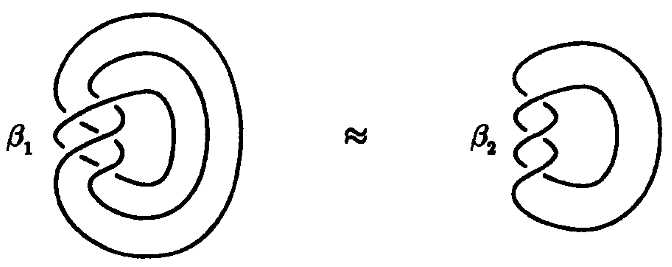
\includegraphics[width=9cm]{Images/exemplo_invariante_alexander.png}
		\end{center}\caption{Dois nós Markov equivalentes.}\label{exemplo invariante de Alexander}
	\end{figure}
	\par\vspace{0.3cm} Como $\beta_1 = (\sigma_1\sigma_2)^2$ e $\beta_2 = \sigma_1^3$ e, por definição, 
	\begin{equation*}
	\varphi_3(\sigma_1) = \begin{bmatrix}
	1-t & t & 0 \\
	1 & 0 & 0 \\
	0 & 0 & 1 
	\end{bmatrix}\text{ e } \varphi_3(\sigma_2) = \begin{bmatrix}
	1 & 0 & 0 \\
	0 & 1-t & t \\
	0 & 1 & 0
	\end{bmatrix}
	\end{equation*}
	\par\vspace{0.3cm} segue que
	\begin{equation*}
	\varphi_3(\sigma_1\sigma_2)^2 = \begin{bmatrix}
	1-t & t-t^2+t^3 & t^2-t^3 \\
	1-t & t-t^2 & t^2 \\
	1 & 0 & 0
	\end{bmatrix}
	\end{equation*}
	\par\vspace{0.3cm} Logo, 
	\begin{equation*}
	\Delta_{\widetilde{\beta}_1}(t) = \det[\varphi_3(\beta_1) - I_3]_{1,1} = \det\begin{bmatrix}
	-1+t-t^2 & t^2 \\
	0 & -1
	\end{bmatrix} = 1-t+t^2
	\end{equation*}
	\par\vspace{0.3cm} Por outro lado, 
	\begin{equation*}
	\varphi_2(\sigma_1) = \begin{bmatrix}
	1-t & t \\
	1 & 0
	\end{bmatrix}\text{ e }\varphi_2(\sigma_1)^3 = \begin{bmatrix}
	1-t+t^2-t^3 & t(1-t+t^2) \\
	1-t+t^2 & t-t^2
	\end{bmatrix}
	\end{equation*}
	\par\vspace{0.3cm} Logo, 
	\begin{equation*}
	\Delta_{\widetilde{\beta}_2}(t) = \det[\varphi_2(\beta_2) - I_2]_{1,1} = -1+t-t^2
	\end{equation*}
	\par\vspace{0.3cm} e, consequentemente, $\Delta_{\widetilde{\beta}_1}(t) = -\Delta_{\widetilde{\beta}_2}(t)$, ou seja, 
	\begin{equation*}
	\Delta_{\widetilde{\beta}_1}(t)\doteq\Delta_{\widetilde{\beta}_2}(t)
	\end{equation*}
	\par\vspace{0.3cm} como esperado.
	\par\vspace{0.3cm} Observe os nós da Figura \eqref{nos exemplo polinomio Alexander}. O nó (a) é o nó $K_a$, fecho de $(\sigma_1\sigma_2^{-1})^2$ em $B_3$ e o nó (b) é o nó $K_b$, fecho de $\sigma_1^n$ em $B_2$.
	\begin{figure}[H]
		\begin{center}
			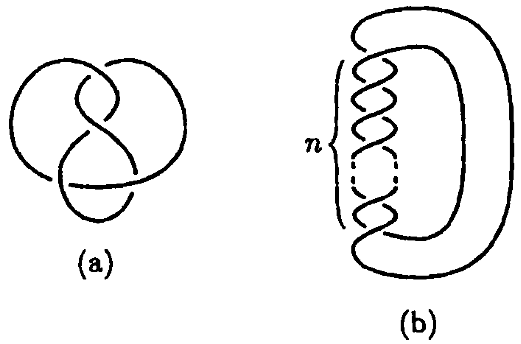
\includegraphics[width=9cm]{Images/no_de_oito_Alexander.png}
		\end{center}\caption{O nó figura oito (a) e um nó com $n$ cruzamentos (b).}\label{nos exemplo polinomio Alexander}
	\end{figure}
	\par\vspace{0.3cm} Por definição, temos
	\begin{equation*}
	\varphi_3(\sigma_1\sigma_2^{-1}) = \begin{bmatrix}
	1-t & t & 0 \\
	1 & 0 & 0 \\
	0 & 0 & 1
	\end{bmatrix}\begin{bmatrix}
	1 & 0 & 0 \\
	0 & 0 & 1 \\
	0 & t^{-1} & 1-t^{-1}
	\end{bmatrix} = \begin{bmatrix}
	1-t & 0 & t \\
	1 & 0 & 0 \\
	0 & t^{-1} & 1-t^{-1}
	\end{bmatrix}
	\end{equation*}
	\par\vspace{0.3cm} Logo,
	\begin{equation*}
	\varphi_3(\sigma_1\sigma_2^{-1})^2 = \begin{bmatrix}
	1-t & 0 & t \\
	1 & 0 & 0 \\
	0 & t^{-1} & 1-t^{-1}
	\end{bmatrix}\begin{bmatrix}
	1-t & 0 & t \\
	1 & 0 & 0 \\
	0 & t^{-1} & 1-t^{-1}
	\end{bmatrix} = \begin{bmatrix}
	(1-t)^2 & 1 & -1 +2t-t^2 \\
	1-t & 0 & t \\
	t^{-1} & t^{-1}-t^{-2} & (1-t^{-1})^2
	\end{bmatrix}
	\end{equation*}
	\par\vspace{0.3cm} Daí, obtemos
	\begin{equation*}
	\Delta_{K_a}(t) = \det[\varphi_3(\sigma_1\sigma_2^{-1})^2 - I_3]_{1,1} = \det\begin{bmatrix}
	-1 & t \\
	t^{-1} - t^{-2} & -1+(1-t^{-1})^2
	\end{bmatrix} = -1+3t^{-1}-t^{-2} \underset{\times (-t^2)}{\doteq} 1-3t+t^2
	\end{equation*}
	\par\vspace{0.3cm} Para o nó $K_b$, temos que
	\begin{equation*}
	\varphi_2(\sigma_1)^n = \begin{bmatrix}
	1-t & t \\
	1 & 0
	\end{bmatrix}^n
	\end{equation*}
	\par\vspace{0.3cm} Como $\varphi_2(\sigma_1)$ tem autovalores $\lambda_{1,2} = 1, -t$ e autovetores $v_{1,2} = (1,1), (-t,1)$, obtemos
	\begin{align*}
	\varphi_2(\sigma_1)^n &= \frac{1}{1+t}\begin{bmatrix}
	1 & -t \\
	1 & 1
	\end{bmatrix}\begin{bmatrix}
	1 & 0 \\
	0 & -t
	\end{bmatrix}^n\begin{bmatrix}
	1 & t \\
	-1 & 1
	\end{bmatrix} \\
	&= \frac{1}{1+t}\begin{bmatrix}
	1 & -t \\
	1 & 1
	\end{bmatrix}\begin{bmatrix}
	1 & 0 \\
	0 & (-t)^n
	\end{bmatrix}\begin{bmatrix}
	1 & t \\
	-1 & 1
	\end{bmatrix} \\
	&= \frac{1}{1+t}\begin{bmatrix}
	1 & (-t)^{n+1} \\
	1 & (-t)^n
	\end{bmatrix}\begin{bmatrix}
	1 & t \\
	-1 & 1
	\end{bmatrix} \\
	&= \frac{1}{1+t}\begin{bmatrix}
	1 - (-t)^{n+1} & t + (-t)^{n+1} \\
	1 - (-t)^n & t + (-t)^n
	\end{bmatrix}
	\end{align*}
	\par\vspace{0.3cm} Daí, temos que
	\begin{align*}
	\Delta_{K_b}(t) = \det[\varphi_2(\sigma_1)^n - I_2]_{1,1} &= \frac{1}{1+t}[t+(-t)^n] - 1 \\
	&= \frac{-1 + (-t)^n}{1+t} \\
	&= -\frac{1 - (-t)^n}{1+t} \\
	&= -\sum_{i=1}^{n}(-t)^{i-1} \\
	&= -(1-t+t^2-\cdots+(-1)^{n-1}t^{n-1}) \\
	&\doteq 1-t+t^2-\cdots+(-1)^{n-1}t^{n-1} 
	\end{align*}
	\par\vspace{0.3cm} Em particular, para $n = 3$ temos o nó de trevo (veja Figura \eqref{no de trevo}) e o polinômio de Alexander $\Delta_{K_b} = 1-t+t^2\underset{\times(t^{-1})}{\doteq} t-1+t^{-1}$.
	\par\vspace{0.3cm} Outro exemplo interessante é o nó toral $K_{a,b}$, cujo polinômio de Alexander é
	\begin{equation*}
	\Delta_{K_{a,b}} = \frac{(1-t^{ab})(1-t)}{(1-t^a)(1-t^b)}
	\end{equation*}
	\par\vspace{0.3cm} Usando a representação de Burau $\varphi_n: B_n\to M(n, \mathbb{Z}[t,t^{-1}])$, podemos definir outras funções. Por exemplo, podemos definir $\overline{\varphi}_n: B_n\to M(n-1, \mathbb{Z}[t,t^{-1}])$ dada por
	\begin{equation*}
	\overline{\varphi}_n(\beta) = \Lambda(t)
	\end{equation*} 
	\par\vspace{0.3cm} sendo $\Lambda(t)$ a matriz definida logo antes do Lema \eqref{lema Alexander}. Daí, afirmamos o seguinte.
	\begin{prop}
		\label{parecido com Burau}
		A função $\overline{\varphi}_n$ é um homomorfismo. %Além disso, para quaisquer $\beta, \gamma\in B_n$, valem as igualdades:
		%\begin{enumerate}
		%\item $\overline{\varphi}_n(\gamma\beta\gamma^{-1}) = %\overline{\varphi}_n(\beta)$
		%\item %$\overline{\varphi}_{n+1}(\beta\sigma_n)(1+t+\cdots+t^%{n-1}) = \overline{\varphi}_n(\beta)(1+t+\cdots+t^n)$
		%\end{enumerate}
	\end{prop}
	\begin{proof}
		Vamos mostrar que $\overline{\varphi}_n$ é homomorfismo. Primeiro, note que se $|i-j|\geq 2$, temos
		\begin{align*}
		(S^{-1}\varphi_n(\sigma_i)S)(S^{-1}\varphi_n(\sigma_j)S) &= S^{-1}\varphi_n(\sigma_i)\varphi_n(\sigma_j)S \\ 
		&= S^{-1}\varphi_n(\sigma_j)\varphi_n(\sigma_i)S \\
		&= (S^{-1}\varphi_n(\sigma_j)S)(S^{-1}\varphi_n(\sigma_i)S)
		\end{align*}
		\par\vspace{0.3cm} Isso implica que
		\begin{align*}
		\left[ \begin{array}{c|c}
		\Lambda(\sigma_i)\Lambda(\sigma_j) & \\
		\hline
		\ast\cdots\ast & 1
		\end{array}\right] = 
		\left[ \begin{array}{c|c}
		\Lambda(\sigma_i) & \\
		\hline
		\ast\cdots\ast & 1
		\end{array}\right]\left[ \begin{array}{c|c}
		\Lambda(\sigma_j) & \\
		\hline
		\ast\cdots\ast & 1
		\end{array}\right]  = \left[\begin{array}{c|c}
		\Lambda(\sigma_j) & \\
		\hline
		\ast\cdots\ast & 1
		\end{array}\right]\left[ \begin{array}{c|c}
		\Lambda(\sigma_i) & \\
		\hline
		\ast\cdots\ast & 1
		\end{array}\right] =  \left[\begin{array}{c|c}
		\Lambda(\sigma_j)\Lambda(\sigma_i) & \\
		\hline
		\ast\cdots\ast & 1
		\end{array}\right]
		\end{align*}
		\par\vspace{0.3cm} ou seja, $\overline{\varphi}_n(\sigma_i)\overline{\varphi}_n(\sigma_j) = \overline{\varphi}_n(\sigma_j)\overline{\varphi}_n(\sigma_i)$ para $|i-j|\geq 2$.
		\par\vspace{0.3cm} De modo similar, vamos mostrar que $\overline{\varphi}_n(\sigma_i)\overline{\varphi}_n(\sigma_{i+1})\overline{\varphi}_n(\sigma_i) = \overline{\varphi}_n(\sigma_{i+1})\overline{\varphi}_n(\sigma_i)\overline{\varphi}_n(\sigma_{i+1})$, ou seja, que $\Lambda(\sigma_i)\Lambda(\sigma_{i+1})\Lambda(\sigma_i) = \Lambda(\sigma_{i+1})\Lambda(\sigma_i)\Lambda(\sigma_{i+1})$. Para isso, basta considerar o caso para $n=3$ pelo mesmo motivo que o fizemos na demonstração da Proposição \eqref{Burau e homomorfismo}. Note que
		\begin{align*}
		(S^{-1}\varphi_3(\sigma_1)S)(S^{-1}\varphi_3(\sigma_2)S)(S^{-1}\varphi_3(\sigma_1)S) = (S^{-1}\varphi_3(\sigma_2)S)(S^{-1}\varphi_3(\sigma_1)S)(S^{-1}\varphi_3(\sigma_2)S)
		\end{align*}
		\par\vspace{0.3cm} Isso implica que 
		\begin{align*}
		\left[\begin{array}{c|c}
		\Lambda(\sigma_1)\Lambda(\sigma_2)\Lambda(\sigma_1) & \\
		\hline 
		\ast\cdots\ast & 1
		\end{array}\right] &= \left[\begin{array}{c|c}
		\Lambda(\sigma_1) & \\
		\hline
		\ast\cdots\ast & 1
		\end{array}\right]\left[\begin{array}{c|c}
		\Lambda(\sigma_2) & \\
		\hline
		\ast\cdots\ast & 1
		\end{array}\right]\left[\begin{array}{c|c}
		\Lambda(\sigma_1) & \\
		\hline
		\ast\cdots\ast & 1
		\end{array}\right] \\ 
		&= \left[\begin{array}{c|c}
		\Lambda(\sigma_2) & \\
		\hline
		\ast\cdots\ast & 1
		\end{array}\right]\left[\begin{array}{c|c}
		\Lambda(\sigma_1) & \\
		\hline
		\ast\cdots\ast & 1
		\end{array}\right]\left[\begin{array}{c|c}
		\Lambda(\sigma_2) & \\
		\hline
		\ast\cdots\ast & 1
		\end{array}\right] \\
		&= \left[\begin{array}{c|c}
		\Lambda(\sigma_2)\Lambda(\sigma_1)\Lambda(\sigma_2) & \\
		\hline
		\ast\cdots\ast & 1
		\end{array}\right]
		\end{align*}
		\par\vspace{0.3cm} como queríamos mostrar. Portanto, $\overline{\varphi}_n$ de fato é homomorfismo.
	\end{proof}
	\par\vspace{0.3cm} Também é possível mostrar que para quaisquer $\beta, \gamma\in B_n$, valem as igualdades:
	\begin{enumerate}
		\item $\overline{\varphi}_n(\gamma\beta\gamma^{-1}) = \overline{\varphi}_n(\beta)$
		\item $\overline{\varphi}_{n+1}(\beta\sigma_n)(1+t+\cdots+t^{n-1}) = \overline{\varphi}_n(\beta)(1+t+\cdots+t^n)$
	\end{enumerate}
	\par\vspace{0.3cm} Desse modo, vamos definir, para uma trança $\beta\in B_n$ arbitrária, 
	\begin{equation*}
	\lambda(\beta) = \frac{\overline{\varphi}_n(\beta)}{1+t+\cdots+t^{n-1}}
	\end{equation*} 
	\par\vspace{0.3cm} Então, $\lambda(\beta)$ é um invariante do fecho de $\beta$, ou seja, se os fechos de $\beta_1\in B_n$ e $\beta_2\in B_m$ representam o mesmo nó $K$, então
	\begin{equation*}
	\frac{\overline{\varphi}_n(\beta_1)}{1+t+\cdots+t^{n-1}} = \frac{\overline{\varphi}_m(\beta_2)}{1+t+\cdots+t^{m-1}}
	\end{equation*}
	\par\vspace{0.3cm} Pode ser mostrado que, na verdade, $\overline{\varphi}_n(\beta)$ é o polinômio de Alexander de $\widetilde{\beta}$.
	\par\vspace{0.3cm} Podemos definir também $\varphi_n^\ast: B_n\to M(n, \mathbb{Z}[t,t^{-1}])$ por
	\begin{equation*}
	\varphi_n^\ast(\sigma_{i_1}^{\varepsilon_1}\sigma_{i_2}^{\varepsilon_2}\cdots\sigma_{i_k}^{\varepsilon_k}) = \varphi_n(\sigma_{i_1}^{\varepsilon_1})^T\varphi_n(\sigma_{i_2}^{\varepsilon_2})^T\cdots\varphi_n(\sigma_{i_k}^{\varepsilon_k})^T
	\end{equation*}
	\par\vspace{0.3cm} De fato, $\varphi_n^\ast$ também é homomorfismo: a demonstração é praticamente idêntica à demonstração da Proposição \eqref{Burau e homomorfismo}, com a pequena diferença de que 
	\begin{equation}
	\label{phi estrela}
	\varphi_n^\ast(\sigma_i) = 
	\left[ 
	\begin{array}{c|cc|c}
	I_{i-1} &  &  & \\
	\hline 
	& 1-t & 1 &  \\
	& t & 0 &  \\ 
	\hline
	&  &  & I_{n-i-1}
	\end{array}
	\right] 
	\end{equation}
	\par\vspace{0.3cm} é a matriz com a qual devemos nos preocupar. Visto que a demonstração é virtualmente idêntica, não a faremos aqui. Ao leitor interessado, basta aplicar os mesmo passos da demonstração da Proposição \eqref{Burau e homomorfismo} à matriz em \eqref{phi estrela}.
	\par\vspace{0.3cm} Além disso, é possível mostrar que 
	\begin{equation*}
	\det[\varphi_n^\ast(\beta) - I_n]_{1,1}\doteq\det[\varphi_n(\beta) - I_n]_{1,1}
	\end{equation*}	
	\par\vspace{0.3cm} logo
	\begin{equation*}
	\Delta_{\widetilde{\beta}}(t) \doteq \det[\varphi_n^\ast(\beta) - I_n]_{1,1}
	\end{equation*}
	\par\vspace{0.3cm} isto é, usar $\varphi_n^\ast(\beta)$ ao invés de $\varphi_n(\beta)$ preserva o polinômio de Alexander a menos de um fator de $\pm t^k$. 
	\par\vspace{0.3cm} Por fim, antes de passarmos ao polinômio de Jones, seja $\beta\in B_n$ e defina um novo polinômio $\nabla_{\widetilde{\beta}}(t)$ na incógnita $\sqrt{t}$ da seguinte forma
	\begin{equation*}
	\nabla_{\widetilde{\beta}}(t) = (-1)^{n-1}t^{-\frac{1}{2}(l(\beta)-n+1)}\det[\varphi_n(\beta) - I_n]_{1,1}
	\end{equation*}
	\par\vspace{0.3cm} É possível mostrar que $\nabla_{\widetilde{\beta}}(t)$ é um invariante de nó. Além disso, se tomarmos $\sigma_p\in B_n$ e, por convenção, fizermos $(\sqrt{t})^2 = t$, então $\nabla$ satisfaz
	\begin{equation}
	\label{polinomio Alexander-Conway}
	\nabla_{\widetilde{\beta\sigma_p}}(t) - \nabla_{\widetilde{\beta\sigma_p^{-1}}}(t) = \left(\frac{1}{\sqrt{t}}- \sqrt{t}\right)\nabla_{\widetilde{\beta}}(t)
	\end{equation}
	\par\vspace{0.3cm} O invariante $\nabla_{\widetilde{\beta}}(t)$ é chamado \textit{polinômio de Alexander-Conway} de $\widetilde{\beta}$, uma vez que foi J.H. Conway quem, por meio de sua (re)descoberta de \eqref{polinomio Alexander-Conway} em 1969, evidenciou essa maneira eficiente de determinar um invariante de um nó (ou \textit{link}). O próprio J.W. Alexander vários anos antes já havia mencionado uma fórmula similiar. Como $\Delta_{\widetilde{\beta}}(t)\doteq\nabla_{\widetilde{\beta}}(t)$ (claramente por um fator de $(-1)^{n-1}t^{-\frac{1}{2}(l(\beta)-n+1)}$), podemos considerar $\nabla_{\widetilde{\beta}}(t)$ como uma reinterpretação do polinômio de Alexander. 
	\par \vspace{0.3cm} Agora, vamos tratar do polinômio de Jones.
	\par\vspace{0.3cm} Em 1984, Vaughan Frederick Randal Jones definiu um novo invariante, hoje nomeado em sua homenagem, o \textit{polinômio de Jones}, denotado por $V_{\widetilde{\beta}}(t)$, para o fecho da trança $\beta$. Assim como o polinômio de Alexander, $V_{\widetilde{\beta}}(t)$ é independente da escolha de $\beta$ no sentido de que se $\widetilde{\beta}_1 = \widetilde{\beta}_2$, temos $V_{\widetilde{\beta}_1}(t) = V_{\widetilde{\beta}_2}(t)$. Antes de definir o invariante de Jones, precisamos de alguns fatos e definições preliminares.
	\begin{deff}
		\label{def prod tensorial}
		Sejam $A = (a_{ij})$ e $B = (a_{kl})$ duas matrizes $p\times q$ e $r\times s$, respectivamente. Então, o produto tensorial de $A$ e $B$, denotado por $A\otimes B$, é a matriz $pr\times qs$ definida por
		\begin{equation*}
		A\otimes B = 
		\begin{bmatrix}
		a_{11}B & a_{12}B & \cdots & a_{1q}B \\
		a_{21}B & a_{22}B & \cdots & a_{2q}B \\
		\vdots & \vdots & \ddots & \vdots \\
		a_{p1}B & a_{p2}B & \cdots & a_{pq}B
		\end{bmatrix}
		\end{equation*}
	\end{deff}
	\par\vspace{0.3cm} Por exemplo, se
	\begin{equation*}
	A = \begin{bmatrix}
	a_{11} & a_{12}
	\end{bmatrix}\text{ e } B = \begin{bmatrix}
	b_{11}\\
	b_{21}
	\end{bmatrix} 
	\end{equation*}
	\par\vspace{0.3cm} então
	\begin{equation*}
	A\otimes B = \begin{bmatrix}
	a_{11}B & a_{12}B
	\end{bmatrix} = \begin{bmatrix}
	a_{11}b_{11} & a_{12}b_{11}\\
	a_{11}b_{21} & a_{12}b_{21}
	\end{bmatrix}
	\end{equation*}
	\par\vspace{0.3cm} Da definição de produto tensorial, segue que 
	\begin{equation}
	\label{propriedade 1 tensorial}
	(A\otimes B)\otimes C = A\otimes(B\otimes C)
	\end{equation}
	\par\vspace{0.3cm} Além disso, note também que se $A$ e $C$ são duas matrizes de ordem $k$ e $B$ e  $D$ são duas matrizes de ordem $l$, então
	\begin{equation}
	\label{propriedade 2 tensorial}
	(A\otimes B)\cdot(C\otimes D) = A\cdot C\otimes B\cdot D
	\end{equation}
	\par\vspace{0.3cm} sendo $(\cdot)$ o produto ordinário de matrizes.
	\par\vspace{0.3cm} De fato, da definição de produto de matrizes, temos que os elementos de $(A\otimes B)(C\otimes D)$ são da forma
	\begin{equation*}
	(A\otimes B)(C\otimes D) = \Bigg(\displaystyle{ \sum_{j=1}^{k}a_{ij}Bc_{js}D}\Bigg) = \Bigg(\displaystyle{ \sum_{j=1}^{k}a_{ij}c_{js}}BD\Bigg) = AC\otimes BD 
	\end{equation*}
	\par\vspace{0.3cm} Agora, dada uma matriz quadrada $M = (a_{ij})$ de ordem $n$, podemos definir o \textit{traço} de $M$, denotado por $\tr(M)$, como
	\begin{equation*}
	\tr(M) = \sum_{i=1}^{n}a_{ii} 
	\end{equation*}
	\par\vspace{0.3cm} ou seja, a soma dos elementos da diagonal principal. O traço de $M$ também pode ser definido em termos do polinômio característico de $M$. Se $\mu_M(\lambda) = \det(M - \lambda I_n)$ é o polinômio característico	de $M$, então $(-1)^{n-1}\tr(M)$ é igual ao coeficiente de $\lambda^{n-1}$ em $\mu_M(\lambda)$. %Vamos demonstrar isso logo mais. 
	\par\vspace{0.3cm} Esse fato também é observado no algoritmo de Fadeev-LeVerrier, um algoritmo recursivo para o cálculo dos coeficientes do polinômio característico de uma matriz. 
	%\begin{prop}
	%	\label{polinomio caracateristico e traco}
	%	Seja $\mu_M(\lambda)$ o polinômio característico da matriz $M$, isto é, $\displaystyle{\mu_M(\lambda) = \sum_{k=0}^{n}c_k\lambda^k}$. Então, $c_n = (-1)^n$ e $c_{n-1} = (-1)^{n-1}\tr(M)$.
	%\end{prop}
	%\begin{proof}
	%	Seja $M = (a_{ij})$. Daí, o polinômio característico de $M$ é dado por
	%	\begin{align*}
	%	\det(M - \lambda I) &=
	%	\begin{vmatrix}
	%	a_{11} - \lambda & a_{12} & \cdots & a_{1\text{ }n-1} & a_{1n} \\
	%	a_{21} & a_{22} - \lambda & \cdots & a_{2\text{ }n-1} & a_{2n} \\
	%	\vdots & \vdots & \ddots & \vdots & \vdots  \\
	%	a_{n-1\text{ }1} & a_{n-1\text{ }2} & \cdots & a_{n-1\text{ }n-1} - \lambda & a_{n\text{ }n-1}   \\
	%	a_{n1} & a_{n2} & \cdots & a_{n\text{ }n-1} & a_{nn} - \lambda 
	%	\end{vmatrix} \\
	%	&= 
	%	\end{align*}
	%\end{proof}
	\par\vspace{0.3cm} Essa reinterpretação pode ser usada como base para a demonstração do seguinte teorema:
	\begin{theorem}
		\label{traco}
		Sejam $P$ uma matriz não singular de ordem $n$ e $M$ uma matriz de ordem $n$. Então, 
		\begin{equation*}
		\tr(M) = \tr(PMP^{-1})
		\end{equation*}
		\par\vspace{0.3cm} e consequentemente
		\begin{equation*}
		\tr(MP) = \tr(PM)
		\end{equation*}
	\end{theorem} 
	\begin{proof}
		Para o primeiro item, usaremos o fato mencionado anteriormente sobre o coeficiente de $\lambda^{n-1}$ em $\mu_M(\lambda)$. Note que 
		\begin{align*}
		\det( PMP^{-1} - \lambda I_n ) &= \det[ PMP^{-1} - \lambda PP^{-1} ] \\
		&= \det[ (PM - \lambda P)P^{-1} ] \\
		&= \det[ (PM - P\lambda)P^{-1} ] \\
		&= \det[ P(M - I_n\lambda)P^{-1} ] \\
		&= \det[ P(M - \lambda I_n)P^{-1} ] \\
		&= \det(M - \lambda I_n)
		\end{align*}
		\par\vspace{0.3cm} Portanto, $M$ e $PMP^{-1}$ têm o mesmo polinômio característico e, consequentemente, segue que $(-1)^{n-1}\tr(M) = (-1)^{n-1}\tr(PMP^{-1})$, ou seja, $\tr(M) = \tr(PMP^{-1})$.
		\par\vspace{0.3cm} Para o segundo item, faremos uma demonstração mais simples e direta. Sejam $P = (a_{ij})$ e $M = (b_{kl})$ duas matrizes de ordem $n$, com $P$ não singular. Então, temos que
		\begin{align*}
		\tr(PM) = \sum_{i=1}^{n}\sum_{j=1}^{n} a_{ij}b_{ji} = \sum_{j=1}^{n}\sum_{i=1}^{n} b_{ji}a_{ij} = \tr(MP)
		\end{align*}
		\par\vspace{0.3cm} Uma demonstração alternativa seria notar que
		\begin{align*}
		\det(MP - \lambda I_n) &= \det(MP - \lambda PP^{-1}) \\
		&= \det[ (M - \lambda P^{-1})P ] \\
		&= \det[ (P^{-1}PM - P{-1}\lambda)P ] \\
		&= \det[ P^{-1}(PM - \lambda I_n)P ] \\
		&= \det(PM - \lambda I_n)
		\end{align*}
		\par\vspace{0.3cm} Portanto, $MP$ e $PM$ têm o mesmo polinômio característico e, consequentemente, segue que $(-1)^{n-1}\tr(MP) = (-1)^{n-1}\tr(PM)$, ou seja, $\tr(MP) = \tr(PM)$.
	\end{proof}
	\par\vspace{0.3cm} Por exemplo, seja 
	\begin{equation}
	\label{parte 1 invariante Jones}
	\mu = \begin{bmatrix}
	1 & 0 \\
	0 & t
	\end{bmatrix}
	\end{equation}
	\par\vspace{0.3cm} Denotando $\underbrace{\mu\otimes\mu\otimes\cdots\otimes\mu}_{n}$ por $\mu^{\otimes n}$, então $\mu^{\otimes n}$ é uma matriz $2^n\times 2^n$ e 
	\begin{equation}
	\label{mi tensor n vezes}
	\tr(\mu^{\otimes n}) = (1+t)^n
	\end{equation}
	\par\vspace{0.3cm} Para perceber esse fato podemos desenvolver $\mu^{\otimes n}$ para alguns valores de $n$ ou então usar o fato de que $\tr(A\otimes B) = \tr(A)\tr(B)$, que pode ser verificado diretamente da definição de produto tensorial. De fato, tomando $A$ e $B$ matrizes de ordem $n$, temos
	\begin{equation*}
	\tr(A\otimes B) = a_{11}\tr(B) + a_{22}\tr(B) + \cdots + a_{nn}\tr(B) = \tr(A)\tr(B)
	\end{equation*}
	\par\vspace{0.3cm} pois, devido à definição de produto tensorial, cada entrada da diagonal de $A\otimes B$ tem a forma $a_{ii}B$, $1\leq i\leq n$. Consequentemente, o traço de $A\otimes B$ tem a forma
	\begin{equation*}
	\sum_{i=1}^{n}a_{ii}(b_{11} + b_{22} + \cdots + b_{nn}) = \tr(B)\sum_{i=1}^{n}a_{ii} = \tr(A)\tr(B)
	\end{equation*}
	\par\vspace{0.3cm} Para que possamos definir o invariante de Jones, precisamos primeiro definir uma nova função $\Phi_n: B_n\to M(2^n, \mathbb{Z}[\sqrt{t}, \frac{1}{\sqrt{t}}])$, baseada na matriz $R$ e em seu inverso. Note que $\Phi_n$ associa uma trança a uma matriz de ordem $2^n$ sobre o módulo $\mathbb{Z}[\sqrt{t}, \frac{1}{\sqrt{t}}]$. 
	\par\vspace{0.3cm} Note também que $\Phi_n$ é similar à representação de Burau: ela também é uma função que associa uma trança a uma matriz de ordem $2^n$. Contudo, aqui o módulo é $\mathbb{Z}[\sqrt{t}, \frac{1}{\sqrt{t}}]$ ao invés de $\mathbb{Z}[t, t^{-1}]$. Além disso, como veremos a seguir, $\Phi_n$ também é definida, em um certo sentido, sobre os geradores $\sigma_i$ do grupo de tranças.
	\par\vspace{0.3cm} Então, sejam
	\begin{equation*}
	R = \begin{bmatrix}
	1 & 0 & 0 & 0 \\
	0 & 0 & -\sqrt{t} & 0 \\
	0 & -\sqrt{t} & 1-t & 0 \\
	0 & 0 & 0 & 1
	\end{bmatrix}\text{ e }R^{-1} = \begin{bmatrix}
	1 & 0 & 0 & 0 \\
	0 & 1 - \frac{1}{t} & -\frac{1}{\sqrt{t}} & 0 \\
	0 & -\frac{1}{\sqrt{t}} & 0 & 0 \\
	0 & 0 & 0 & 1
	\end{bmatrix}
	\end{equation*}
	\par\vspace{0.3cm} Como antes, usamos a convenção de que $(\sqrt{t})^2 = t$.
	\par\vspace{0.3cm} Para um $i$ arbitrário, definimos $\Phi_n(\sigma_i^{\varepsilon})$ como a seguinte matriz de ordem $2^n$:
	\begin{equation}
	\label{Phi invariante Jones}
	\Phi_n(\sigma_i^{\varepsilon}) = \underbrace{I_2\otimes\cdots\otimes I_2}_{i-1}\otimes R^{\varepsilon}\otimes\underbrace{I_2\otimes\cdots\otimes I_2}_{n-i-1}
	\end{equation}
	\par\vspace{0.3cm} sendo $\varepsilon=\pm1$ e $I_2$ a matriz identidade de ordem 2. Note que, de fato $\Phi_n(\sigma_i^{\varepsilon})$ tem ordem $2^{i-1}\cdot4\cdot2^{n-i-1} = 2^n$.
	\par\vspace{0.3cm} De \eqref{Phi invariante Jones} podemos definir
	\begin{equation}
	\label{parte 2 invariante Jones}
	\Phi_n(\beta) = \Phi_n(\sigma_{i_1}^{\varepsilon_1})\cdots\Phi_n(\sigma_{i_k}^{\varepsilon_k})\in M(2^n, \mathbb{Z}[\sqrt{t}, \frac{1}{\sqrt{t}}])
	\end{equation}
	\par\vspace{0.3cm} para $\beta = \sigma_{i_1}^{\varepsilon_1}\cdots\sigma_{i_k}^{\varepsilon_k}$, com $1\leq i_1, \dots, i_k\leq n-1$ e $\varepsilon_j=\pm1$. 
	\par\vspace{0.3cm} A função
	\begin{equation*}
	\xi(\beta) = \frac{t^{\nu}\tr(\Phi_n(\beta)\mu^{\otimes n})}{1+t}
	\end{equation*}
	\par\vspace{0.3cm} sendo $\nu = \displaystyle{ \frac{1}{2}\big(l(\beta) - n + 1\big) }$, é o invariante de Jones. Essa afirmação será propriamente demonstrada no Teorema \eqref{polinomio de Jones}, a partir dos dois lemas a seguir.
	\begin{lemma}
		\label{lema 1 Jones}
		A função $\Phi_n$ é um homomorfismo de $B_n$ em $M(2^n, \mathbb{Z}[\sqrt{t}, \frac{1}{\sqrt{t}}])$
	\end{lemma}
	\begin{proof}
		Precisamos mostrar que 
		\begin{enumerate}
			\item $\Phi_n(\sigma_i\sigma_j) = \Phi_n(\sigma_j\sigma_i)$ se $|i-j|\geq 2$
			\item $\Phi_n(\sigma_i\sigma_{i+1}\sigma_i) = \Phi_n(\sigma_{i+1}\sigma_i\sigma_{i+1})$ para $i=1,2,\dots, n-2$
		\end{enumerate}
		\par\vspace{0.3cm} Vamos começar com 1. Sem perda de generalidade, podemos supor $j>i+1$. Então, de \eqref{propriedade 1 tensorial} e \eqref{propriedade 2 tensorial} tomando $I = I_2$, temos
		\begin{align*}
		\Phi_n(\sigma_i\sigma_j) &= \Phi_n(\sigma_i)\Phi_n(\sigma_j) \\
		&= (I^{\otimes i-1} \otimes R \otimes I^{\otimes n-i-1})( I^{\otimes j-1} \otimes R \otimes I^{\otimes n-j-1} ) \\
		&= ( I^{\otimes i-1} \otimes R \otimes I^{\otimes j-i-2}\otimes I^{\otimes 2} \otimes I^{\otimes n-j-1}  ) \times (I^{\otimes i-1} \otimes I^{\otimes 2} \otimes I^{\otimes j-i-2} \otimes R \otimes I^{\otimes n-j-1} ) \\
		&=  [(I^{\otimes i-1} \otimes R \otimes I^{\otimes j-i-2})\underbrace{\times(I^{\otimes i-1}\otimes I^{\otimes 2} \otimes I^{\otimes j-i-2})}_{I^{\otimes j-1} = I_{2^{j-1}}}]\otimes [\underbrace{(I^{\otimes 2} \otimes I^{\otimes n-j-1})}_{I^{\otimes n-j+1} = I_{2^{n-j+1}}  }\times(R \otimes I^{\otimes n-j-1})] \\
		&= I^{\otimes i-1} \otimes R \otimes I^{\otimes j-i-2} \otimes R \otimes I^{\otimes n-j-1}
		\end{align*} 
		\par\vspace{0.3cm} De modo similar, obtemos
		\begin{equation*}
		\Phi_n(\sigma_j\sigma_i) = I^{\otimes i-1} \otimes R \otimes I^{\otimes j-i-2} \otimes R \otimes I^{\otimes n-j-1}
		\end{equation*}
		\par\vspace{0.3cm} Vamos demonstrar 2 agora. Primeiro, note que de \eqref{propriedade 1 tensorial} e \eqref{propriedade 2 tensorial} temos
		\begin{align*}
		\Phi_n(\sigma_i\sigma_{i+1}\sigma_i) &= (I^{\otimes i-1} \otimes R \otimes I^{\otimes n-i-1}) (I^{\otimes i} \otimes R \otimes I^{\otimes n-i-2}) (I^{\otimes i-1} \otimes R \otimes I^{\otimes n-i-1}) \\
		&= (I^{\otimes i-1} \otimes (R\otimes I) \otimes I^{\otimes n-i-2}) (I^{\otimes i-1} \otimes (I\otimes R) \otimes I^{\otimes n-i-2}) (I^{\otimes i-1} \otimes (R \otimes I) \otimes I^{\otimes n-i-2}) \\
		&= I^{\otimes i-1}[(R \otimes I)(I \otimes R)(R \otimes I)]I^{\otimes n-i-2}
		\end{align*}
		\par\vspace{0.3cm} enquanto que
		\begin{align*}
		\Phi_n(\sigma_{i+1}\sigma_i\sigma_{i+1}) = I^{\otimes i-1}[(I \otimes R)(R \otimes I)(I \otimes R)]I^{\otimes n-i-2}
		\end{align*}
		\par\vspace{0.3cm} Portanto, basta mostrar que
		\begin{equation*}
		(R \otimes I)(I \otimes R)(R \otimes I) = (I \otimes R)(R \otimes I)(I \otimes R)
		\end{equation*}
		\par\vspace{0.3cm} o que pode ser verificado por uma computação direta (mas entediante).
	\end{proof}
	\begin{lemma}
		\label{lema 2 Jones}
		Seja $\xi(\beta)$ a função definida acima (e também no Teorema \eqref{polinomio de Jones}). Então, ela satisfaz as seguintes condições:
		\begin{enumerate}
			\item Para quaisquer tranças $\beta, \gamma\in B_n$, $\xi(\gamma\beta\gamma^{-1})=\xi(\beta)$;
			\item Para uma trança $\beta\in B_n$ qualquer e para as tranças $\beta\sigma_n^{\pm1}$, $\xi(\beta) = \xi(\beta\sigma_n) = \xi(\beta\sigma_n^{-1})$.
		\end{enumerate}
	\end{lemma}
	\begin{proof}
		Vamos mostrar o item 1. Podemos escrever $\beta\in B_n$ como $\beta = \sigma_{i_1}^{\varepsilon_1}\cdots\sigma_{i_k}^{\varepsilon_k}$. Então,
		\begin{equation*}
		\Phi_n(\beta) = R_{i_1}^{\varepsilon_1}\cdots R_{i_k}^{\varepsilon_k}
		\end{equation*}
		\par\vspace{0.3cm} sendo 
		\begin{equation*}
		R_{i_j}^{\varepsilon_j} = \underbrace{I\otimes \cdots \otimes I}_{i_j - 1}\otimes R^{\varepsilon_j}\otimes \underbrace{I\otimes \cdots\otimes I}_{n-i_j-1}.
		\end{equation*} 
		\par\vspace{0.3cm} Para qualquer trança $\beta\in B_n$
		\begin{equation*}
		\Phi_n(\beta)\mu^{\otimes n} = \mu^{\otimes n}\Phi_n(\beta)
		\end{equation*}
		\par\vspace{0.3cm} Para ver isso, note que basta mostrarmos que
		\begin{equation}
		\label{R mi duas vezes}
		R^{\varepsilon}\mu^{\otimes 2} = \mu^{\otimes 2}R^{\varepsilon}
		\end{equation}
		\par\vspace{0.3cm} sendo $\varepsilon=\pm1$, devido ao fato de que se $R^{\varepsilon}$ comuta com $\mu^{\otimes 2}$, então ele também comuta com $\mu^{\otimes n}$, pois $\mu^{\otimes n}$ é formada por blocos de $\mu^{\otimes 2}$ multiplicados por fatores $t^k$. Calculando, temos
		\begin{align*}
		R\mu^{\otimes 2} &= \begin{bmatrix}
		1 & 0 & 0 & 0 \\
		0 & 0 & -\sqrt{t} & 0 \\
		0 & -\sqrt{t} & 1-t & 0 \\
		0 & 0 & 0 & 1
		\end{bmatrix}\begin{bmatrix}
		1 \\
		& t \\
		& & t \\
		& & & t^2
		\end{bmatrix} \\
		&= \begin{bmatrix}
		1 & 0 & 0 & 0 \\
		0 & 0 & -t\sqrt{t} & 0 \\
		0 & -t\sqrt{t} & (1-t)t &  0 \\
		0 & 0 & 0 & t^2
		\end{bmatrix} \\
		&= \begin{bmatrix}
		1 \\
		& t \\
		& & t \\
		& & & t^2
		\end{bmatrix}\begin{bmatrix}
		1 & 0 & 0 & 0 \\
		0 & 0 & -\sqrt{t} & 0 \\
		0 & -\sqrt{t} & 1-t & 0 \\
		0 & 0 & 0 & 1
		\end{bmatrix} 
		= \mu^{\otimes 2}R
		\end{align*}
		\par\vspace{0.3cm} e também
		\begin{align*}
		R^{-1}\mu^{\otimes 2} &= \begin{bmatrix}
		1 & 0 & 0 & 0 \\
		0 & 1 - \frac{1}{t} & -\frac{1}{\sqrt{t}} & 0 \\
		0 & -\frac{1}{\sqrt{t}} & 0 & 0 \\
		0 & 0 & 0 & 1
		\end{bmatrix}\begin{bmatrix}
		1 \\
		& t \\
		& & t \\
		& & & t^2
		\end{bmatrix} \\
		&= \begin{bmatrix}
		1 & 0 & 0 & 0 \\
		0 & t-1 & -\frac{t}{\sqrt{t}} & 0 \\
		0 & -\frac{t}{\sqrt{t}} & 0 &  0 \\
		0 & 0 & 0 & t^2
		\end{bmatrix} \\
		&= \begin{bmatrix}
		1 \\
		& t \\
		& & t \\
		& & & t^2
		\end{bmatrix}\begin{bmatrix}
		1 & 0 & 0 & 0 \\
		0 & 1 - \frac{1}{t} & -\frac{1}{\sqrt{t}} & 0 \\
		0 & -\frac{1}{\sqrt{t}} & 0 & 0 \\
		0 & 0 & 0 & 1
		\end{bmatrix} = \mu^{\otimes 2}R^{-1}
		\end{align*}
		\par\vspace{0.3cm} Daí, sendo $\beta, \gamma\in B_n$ arbitrárias, 
		\begin{align*}
		\Phi_n(\gamma\beta\gamma^{-1}) \mu^{\otimes n} &= \Phi_n(\gamma)\Phi_n(\beta)\Phi_n(\gamma^{-1})\mu^{\otimes n} \\
		&= \Phi_n(\gamma)(\Phi_n(\beta)\mu^{\otimes n})\Phi_n(\gamma^{-1})
		\end{align*}
		\par\vspace{0.3cm} Logo, como $\Phi_n$ é homomorfismo e pelo Teorema \eqref{traco}, obtemos
		\begin{align*}
		\tr(\Phi_n(\gamma\beta\gamma^{-1}) \mu^{\otimes n})	&= \tr(\Phi_n(\gamma)(\Phi_n(\beta)\mu^{\otimes n})\Phi_n^{-1}(\gamma)) \\
		&= \tr(\Phi_n(\beta)\mu^{\otimes n})
		\end{align*}
		\par\vspace{0.3cm} Como $l(\gamma\beta\gamma^{-1}) = l(\beta)$, segue que
		\begin{equation*}
		\xi(\gamma\beta\gamma^{-1}) = \xi(\beta)
		\end{equation*}
		\par\vspace{0.3cm} e concluímos a demonstração de 1. Agora, 2.
		\par\vspace{0.3cm} Suponha $\beta\in B_n$. Então, $\Phi_n(\beta) = M\in M(2^n, \mathbb{Z}[\sqrt{t}, \frac{1}{\sqrt{t}}])$. Precisamos computar a matriz $\Phi_{n+1}(\beta\sigma_n)$, de ordem $2^{n+1}$. De \eqref{parte 2 invariante Jones}, temos
		\begin{equation*}
		\Phi_{n+1}(\beta\sigma_n) = \Phi_{n+1}(\beta)\Phi_{n+1}(\sigma_n)
		\end{equation*}
		\par\vspace{0.3cm} Além disso, de \eqref{Phi invariante Jones}, temos
		\begin{equation*}
		\Phi_{n+1}(\beta) = \Phi_n(\beta)\otimes I \text{ e }\Phi_{n+1}(\sigma_n) = I^{\otimes n-1}\otimes R
		\end{equation*}
		\par\vspace{0.3cm} Se fizermos $\Phi_n(\beta) = M = ||a_{ij}||$, então
		\begin{equation*}
		\Phi_{n+1}(\beta\sigma_n)\mu^{\otimes n+1} = (M\otimes I)(I^{\otimes n-1}\otimes R)(\underbrace{\mu\otimes\cdots\otimes\mu}_{n+1})
		\end{equation*}
		\par\vspace{0.3cm} enquanto que
		\begin{equation*}
		\Phi_n(\beta)\mu^{\otimes n} = M(\underbrace{\mu\otimes\cdots\otimes\mu}_{n})
		\end{equation*}
		\par\vspace{0.3cm} Agora, se escrevermos 
		\begin{align*}
		\mu^{\otimes n} = \begin{bmatrix}
		b_1 \\
		& b_2 \\
		& & \ddots \\
		& & & b_{2^n}
		\end{bmatrix}
		\end{align*}
		\par\vspace{0.3cm} então 
		\begin{equation*}
		\tr(\Phi_n(\beta)\mu^{\otimes n}) = \sum_{i=1}^{2^n}a_{ii}b_i
		\end{equation*}
		\par\vspace{0.3cm} Os $b_i$ têm a forma
		\begin{align*}
		b_1 = 1&, b_2 = t \\
		\text{para }p\geq 1, b_i = tb_p \text{ se }i=2p &\text{ e } b_i = b_p \text{ se }i=2p-1 
		\end{align*}
		\par\vspace{0.3cm} Isso pode ser verificado por indução em $n$. De fato, devido à definição de $\mu$ é imediato que $b_1 = 1$ e $b_2 = t$. Suponha, então, que essa forma é válida para $p = 2^{n-1}$, ou seja, para $\mu^{\otimes n-1 }$. Assim, segue da definição de produto tensorial que para $\mu^{\otimes n}$ a mesma forma se manterá.
		\par\vspace{0.3cm} Como consequência imediata segue o fato de que se $i = 2^kq$, com $q =2r - 1$, então $b_i = t^kb_q$. Em particular, $b_{2^k} = t^k$.
		\par\vspace{0.3cm} Como $\mu^{\otimes n+1}$ é uma matriz diagonal, para calcularmos $\tr( (\Phi_{n+1}(\beta\sigma_n))\mu^{\otimes n+1} )$ basta conhecer as entradas da diagonal de $\Phi_{n+1}(\beta\sigma_n)$, ou seja, as entradas da diagonal de $(M\otimes I)(I^{\otimes n-1}\otimes R)$. 
		\par\vspace{0.3cm} Sabemos que $I^{\otimes n-1}\otimes R$ é uma matriz diagonal de ordem $2^{n+1}$ da forma
		\begin{align*}
		I^{\otimes n-1}\otimes R = \left.\begin{bmatrix}
		R \\
		& R \\
		& & \ddots \\
		& & & R
		\end{bmatrix} \right \} 2^{n-1}\text{ blocos}
		\end{align*}
		\par\vspace{0.3cm} Portanto, cada uma das entradas da diagonal de $\Phi_{n+1}(\beta\sigma_n)$ vêm do produto
		\begin{align*}
		\left( \begin{bmatrix}
		a_{2i-1,2i-1} & a_{2i-1, 2i} \\
		a_{2i,2i-1} & a_{2i, 2i}
		\end{bmatrix}\otimes I \right)R
		\end{align*}
		\par\vspace{0.3cm} que, ignorando todas as entradas fora da diagonal, pode ser expandido como segue
		\begin{align*}
		\begin{bmatrix}
		a_{2i-1, 2i-1} \\
		& 0 \\
		& & a_{2i,2i}(1-t) \\
		& & & a_{2i,2i}
		\end{bmatrix}
		\end{align*}
		\par\vspace{0.3cm} Usando a forma dos $b_i$ encontrada anteriormente, podemos computar $\tr((\Phi_{n+1}(\beta\sigma_n))\mu^{\otimes n+1})$
		\begin{align*}
		\tr((\Phi_{n+1}(\beta\sigma_n))\mu^{\otimes n+1}) &= \sum_{i=1}^{2^{n-1}} \left\{ a_{2i-1,2i-1}b_{4i-3} + a_{2i,2i}(1-t)b_{4i-1} + a_{2i,2i}b_{4i} \right\} \\
		&= \sum_{i=1}^{2^{n-1}} \left\{ a_{2i-1,2i-1}b_{2(2i-1)-1} + a_{2i,2i}(1-t)b_{2(2i)-1} + a_{2i,2i}b_{2(2i)} \right\} \\
		&= \sum_{i=1}^{2^{n-1}} \left\{ a_{2i-1,2i-1}b_{2i-1} + a_{2i,2i}[(1-t)b_{2i} + tb_{2i}] \right\} \\
		&= \sum_{i=1}^{2^{n-1}} \left\{ a_{2i-1,2i-1}b_{2i-1} + a_{2i,2i}b_{2i} \right\} \\
		&= \sum_{j=1}^{2^n}a_{jj}b_j \\
		&= \tr ( \Phi_n(\beta)\mu^{\otimes n}  )
		\end{align*}
		\par\vspace{0.3cm} Uma vez que $l(\beta\sigma_n) = l(\beta) + 1$, segue que
		\begin{equation*}
		\xi(\beta\sigma_n) = \xi(\beta)
		\end{equation*}
		\par\vspace{0.3cm} pois os traços são iguais e o expoente de $t$ em $\xi(\beta\sigma_n)$ é $\displaystyle{ \frac{1}{2}(l(\beta) + 1 - (n +1) + 1) = \frac{1}{2}( l(\beta) - n + 1 ) }$, que é igual ao expoente de $t$ em $\xi(\beta)$.
		\par\vspace{0.3cm} De modo similar, para $\sigma_n^{-1}$ no lugar de $\sigma_n$, basta substituirmos $R$ por $R^{-1}$. Desse modo, 
		\begin{equation*}
		\Phi_{n+1}(\beta\sigma_n^{-1})\mu^{\otimes n+1} = (M\otimes I)(I^{\otimes n-1}\otimes R^{-1})\mu^{\otimes n+1}
		\end{equation*}
		\par\vspace{0.3cm} Como antes, para calcular $\tr ( (\Phi_{n+1}(\beta\sigma_n^{-1}))\mu^{\otimes n+1} )$ é suficiente saber as entradas da diagonal de $ \Phi_{n+1}(\beta\sigma_n^{-1}) $, ou seja, as entradas da diagonal de $(M\otimes I)(I^{\otimes n-1}\otimes R^{-1})$. 
		\par\vspace{0.3cm} Sabemos que $I^{\otimes n-1}\otimes R^{-1}$ é uma matriz diagonal de ordem $2^{n+1}$, podendo ser escrita como
		\begin{align*}
		I^{\otimes n-1}\otimes R^{-1} = \left. \begin{bmatrix}
		R^{-1} \\
		& R^{-1} \\
		& & \ddots \\
		& & & R^{-1}
		\end{bmatrix} \right\} 2^{n-1}\text{ blocos}
		\end{align*}
		\par\vspace{0.3cm} Consequentemente, as entradas diagonais de $\Phi_{n+1}(\beta\sigma_n^{-1})$ vêm do produto
		\begin{align*}
		\left( \begin{bmatrix}
		a_{2i-1,2i-1} & a_{2i-1,2i} \\
		a_{2i,2i-1} & a_{2i,2i} 
		\end{bmatrix}\otimes I \right)R^{-1}
		\end{align*}
		\par\vspace{0.3cm} que, ignorando as entradas não diagonais, pode ser expandida como
		\begin{align*}
		\begin{bmatrix}
		a_{2i-1,2i-1} \\
		& a_{2i-1,2i-1}(1-\frac{1}{t}) \\
		& & 0 \\
		& & & a_{2i,2i}
		\end{bmatrix}
		\end{align*}
		\par\vspace{0.3cm} Daí, usando a forma dos $b_i$ encontrada anteriormente, temos
		\begin{align*}
		\tr((\Phi_{n+1}(\beta\sigma_n^{-1}))\mu^{\otimes n+1}) &= \sum_{i=1}^{2^{n-1}} \left\{ a_{2i-1,2i-1}b_{4i-3} + a_{2i-1,2i-1}\left(1-\frac{1}{t}\right)b_{4i-2} + a_{2i,2i}b_{4i} \right\} \\
		&= \sum_{i=1}^{2^{n-1}} \left\{ a_{2i-1,2i-1}b_{2(2i-1)-1} + a_{2i-1,2i-1}\left(1-\frac{1}{t}\right)b_{2(2i-1)} + a_{2i,2i}b_{2(2i)} \right\} \\
		&= \sum_{i=1}^{2^{n-1}} \left\{ a_{2i-1,2i-1}[b_{2i-1} + tb_{2i-1} - b_{2i-1}] + a_{2i,2i}tb_{2i}\right\} \\
		&= t\sum_{i=1}^{2^{n-1}} \left\{ a_{2i-1,2i-1}b_{2i-1} + a_{2i,2i}b_{2i} \right\} \\
		&= t\sum_{j=1}^{2^n}a_{jj}b_j \\
		&= t\tr ( \Phi_n(\beta)\mu^{\otimes n}  )
		\end{align*}
		\par\vspace{0.3cm} Como $l(\beta\sigma_n^{-1}) = l(\beta) - 1$, temos
		\begin{align*}
		\xi(\beta\sigma_n^{-1}) &=  \frac{\tr(\Phi_n(\beta)\mu^{\otimes n}) }{ 1+t }t\cdot t^{ \frac{1}{2}(l(\beta) -1 - (n+1) + 1  ) } \\
		&= \frac{\tr(\Phi_n(\beta)\mu^{\otimes n}) }{ 1+t }t^{ \frac{1}{2}(l(\beta)- n+1) } \\
		&= \xi(\beta)
		\end{align*}
		\par\vspace{0.3cm} e finalizamos a demonstração.
	\end{proof}
	\par\vspace{0.3cm} Agora podemos demonstrar o teorema desejado.
	\begin{theorem}
		\label{polinomio de Jones}
		Com a função $\Phi_n$ definida em \eqref{Phi invariante Jones} e \eqref{parte 2 invariante Jones} e a matriz $\mu$ definida em \eqref{parte 1 invariante Jones}, temos que
		\begin{equation}
		\label{invariante Jones}
		\xi(\beta) = \frac{t^{\nu}\tr(\Phi_n(\beta)\mu^{\otimes n})}{1+t}
		\end{equation}
		\par\vspace{0.3cm} com $\nu = \displaystyle{ \frac{1}{2}(l(\beta) - n + 1) }$, é um invariante de $\widetilde{\beta}$, independente da escolha de $\beta$. Em outras palavras, se $\widetilde{\beta_1}\approx\widetilde{\beta_2}$, para $\beta_1\in B_n$ e $\beta_2\in B_m$, então $\xi(\beta_1) = \xi(\beta_2)$. Esse invariante de nó é chamado polinômio de Jones de um nó (ou link) e denotado por $V_{\widetilde{\beta}}(t)$.
	\end{theorem}
	\begin{proof}
		Suponha que os fechos de $\beta$ e $\beta'$, $\widetilde{\beta}$ e $\widetilde{\beta'}$ respectivamente, são equivalentes. Então, pelo Teorema \eqref{teorema de Markov}, $\beta\underset{M}{\sim}\beta'$, i.e., existe uma sequência finita
		\begin{equation*}
		\beta = \beta_0\to\beta_1\to\cdots\to\beta_m=\beta'
		\end{equation*}
		\par\vspace{0.3cm} tal que $\beta_{i+1}$ é obtida de $\beta_i$, para $i = 0,1,\dots,m-1$, aplicando um dos movimentos de Markov $M_1^{\pm1}$ e $M_2^{\pm1}$.
		\par\vspace{0.3cm} Note que se $\beta$ e $\beta'$ são tranças equivalentes, então $\beta = \beta'$ como tranças de $n$ cordas e, portanto, $\Phi_n(\beta) = \Phi_n(\beta')$. Como $l(\beta) = l(\beta')$ (pois $l(\beta)$ é um invariante de tranças), segue que $\xi(\beta) = \xi(\beta')$.
		\par\vspace{0.3cm} Se $\beta_{i+1}$ é conjugada de $\beta_i$, ou seja, se $\beta_i\xrightarrow{M_1}\beta_{i+1}$ ou $\beta_i\xrightarrow{M_1^{-1}}\beta_{i+1}$, então pelo item 1 do Lema \eqref{lema 2 Jones} temos $\xi(\beta_i) = \xi(\beta_{i+1})$.
		\par\vspace{0.3cm} Por outro lado, se $\beta_i\xrightarrow{M_2}\beta_{i+1}$ ou $\beta_i\xrightarrow{M_2^{-1}}\beta_{i+1}$, então pelo item 2 do Lema \eqref{lema 2 Jones}, temos $\xi(\beta_i) = \xi(\beta_{i+1})$.
		\par\vspace{0.3cm} Portanto, $\xi(\beta) = \xi(\beta')$, como queríamos mostrar.
	\end{proof}
	\par\vspace{0.3cm} Para $n=2$, por exemplo, temos $\Phi_2(\sigma_1) = R$ e $\tr( \Phi_2(\sigma_1)\mu^{\otimes 2} ) = \tr(R\mu^{\otimes 2}) = 1+t$ (veja o cálculo de \eqref{R mi duas vezes}). Daí, como $l(\sigma_1) = 1$, temos $V_{\widetilde{\sigma_1}}(t) = \xi(\sigma_1) = \displaystyle{\frac{t^{\frac{1}{2}(1-2+1)} 
			(1+t) }{1+t}} = 1$.
	\par\vspace{0.3cm} Para $n=3$ e $\beta = \sigma_1\sigma_2$ em $B_3$, é trabalhoso, mas não muito difícil, mostrar que
	\begin{equation*}
	\tr(\Phi_3(\sigma_1\sigma_2)\mu^{\otimes 3}) = \tr( (R\otimes I)(I\otimes R) \mu^{\otimes 3} ) = 1+t
	\end{equation*} 
	\par\vspace{0.3cm} Como $l(\beta) = 2$, temos
	\begin{align*}
	V_{\widetilde{\beta}}(t) = \frac{t^{\frac{1}{2}(2-3+1)} (1+t)  }{1+t} = 1
	\end{align*}
	\par\vspace{0.3cm} o que era esperado, pois $\sigma_1$ em $B_2$ e $\sigma_1\sigma_2$ em $B_3$ representam o nó trivial.
	\par\vspace{0.3cm} Se considerarmos a trança trivial $\beta =1_n\in B_n$, então $\Phi_n(\beta) = I^{\otimes n}$ e, daí, usando $\eqref{mi tensor n vezes}$, temos
	\begin{equation*}
	\tr( \Phi_n(\beta)\mu^{\otimes n} ) = \tr(\mu^{\otimes n}) = (1+t)^n
	\end{equation*} 
	\par\vspace{0.3cm} Uma vez que $l(\beta) = 0$,
	\begin{align*}
	V_{\widetilde{\beta}}(t) &= \frac{t^{-\frac{n-1}{2}} (1+t)^n}{1+t} \\
	&= \left( \frac{1}{\sqrt{t}} + \sqrt{t} \right)^{n-1}
	\end{align*}
	\par\vspace{0.3cm} Se fizermos $t=1$, então, como $\sqrt{1}$ é a raiz primitiva da unidade (i.e., $e^{i\pi} = -1$), temos $\sqrt{t} = -1$ e, portanto
	\begin{equation}
	\label{polinomio de jones tranca trivial}
	V_{\widetilde{\beta}}(1) = V_{\widetilde{1_n}}(1) = (-2)^{n-1}
	\end{equation}
	\par\vspace{0.3cm} Em geral, computar $V_{\widetilde{\beta}}(t)$ para uma trança $\beta$ arbitrária é algo trabalhoso.
	\par\vspace{0.3cm} Outros exemplos são os polinômios de Jones para o nó figura oito 
	\begin{equation*}
	V_{\widetilde{\beta}}(t) = t^2 - t + 1 - t^{-1} + t^{-2}  
	\end{equation*}
	\par\vspace{0.3cm} e para os nós torais
	\begin{equation*}
	V_{K_{p,q}}(t) = \frac{1-t^{p+1}-t^{q+1} + t^{p+q}}{1-t^2}t^{(p-1)(q-1)/2}
	\end{equation*}
	\subsubsection{Alexander vs Jones}
	\hspace{12pt} Agora, vamos falar um pouco das diferenças entre os dois invariantes de nós definidos anteriormente, os polinômios de Alexander e Jones.
	\par\vspace{0.3cm} Uma primeira diferença notável entre os dois polinômios é que, por exemplo, para o \textit{link} $K = \widetilde{\sigma_1\sigma_3}$ em $B_4$, temos $\Delta_K(t) = 0$ (não é muito trabalhoso calcular). Contudo, vamos provar que $V_K(t)\neq 0$ qualquer que seja o \textit{link} ou nó $K$. Portanto, devido a essa observação, podemos dizer que nesse aspecto $V_K(t)$ é um invariante ``mais forte'' que $\Delta_K(t)$. 
	\par\vspace{0.3cm} Começamos com um fato acerca do polinômio de Alexander.
	\begin{prop}
		\label{polinomio de Alexander para t=1}
		Se $K$ é um nó, então $|\Delta_K(1)|=1$.
	\end{prop}
	\begin{proof}
		Seja $\sigma_i$ um gerador de $B_n$ e defina $\widehat{\varphi}_n$ como
		\begin{equation*}
		\widehat{\varphi}_n(\sigma_i) = \varphi_n(\sigma_i)|_{t=1} = \left[ \begin{array}{c|cc|c}
		I_{i-1} & & & \\
		\hline
		& 0 & 1 & \\
		& 1 & 0 & \\
		\hline 
		& & & I_{n-i-1}
		\end{array}\right] 
		\end{equation*}
		\par\vspace{0.3cm} Daí, temos $\widehat{\varphi}_n(\sigma_i^2) = I_n$. Portanto, $\widehat{\varphi}_n$ define um homomorfismo de $B_n/\langle \sigma_i^2 \rangle$ em $M(n, \mathbb{Z})$. Como $B_n/\langle \sigma_i^2 \rangle\cong S_n$, $\widehat{\varphi}_n$ é um homomorfismo de $S_n$ em $M(n,\mathbb{Z})$. Contudo, o isomorfismo $B_n/\langle \sigma_i^2 \rangle\cong S_n$ é dado pela permutação $\pi(\beta)$ associada à trança $\beta\in B_n$. Logo, se $\pi(\beta) = \pi(\beta')$ então $\widehat{\varphi}_n(\beta) = \widehat{\varphi}_n(\beta')$, ou seja
		\begin{equation}
		\label{igualdade de modulos}
		|\Delta_{\widetilde{\beta}}(1)| = |\Delta_{\widetilde{\beta'}}(1)|
		\end{equation}
		\par\vspace{0.3cm} Como $\widetilde{\beta}$ é um nó, $\pi(\beta)$ é uma permutação de ordem $n$. Daí, segue que tomando uma conjugação apropriada de $\beta$, temos
		\begin{equation*}
		\pi(\gamma\beta\gamma^{-1}) = (123\dots n)
		\end{equation*}
		\par\vspace{0.3cm} Então, seja $\beta' = \sigma_{n-1}\sigma_{n-2}\cdots\sigma_2\sigma_1$. Consequentemente, $\pi(\beta') = (123\dots n)$ e, por \eqref{igualdade de modulos}
		\begin{equation*}
		| \Delta_{\widetilde{\gamma\beta\gamma^{-1}}}(1) | = | \Delta_{\widetilde{\beta'}}(1) |
		\end{equation*}
		\par\vspace{0.3cm} Mas $\widetilde{\gamma\beta\gamma^{-1}}$ é o mesmo nó que $\widetilde{\beta}$, devido ao movimento de Markov tipo 1, $M_1$. Fazendo $K = \widetilde{\beta}$ e $K' = \widetilde{\beta'}$, temos
		\begin{equation*}
		|\Delta_K(1)| = |\Delta_{K'}(1)|
		\end{equation*} 
		\par\vspace{0.3cm} Como $K'$ é o nó trivial, segue que $\Delta_{K'}(t) = 1$ e, em particular, que $\Delta_{K'}(1) = 1$. Portanto, para qualquer nó $K$,
		\begin{equation*}
		|\Delta_K(1)| = |\Delta_{K'}(1)| = 1
		\end{equation*}
	\end{proof}
	\par\vspace{0.3cm} Note que na Proposição \eqref{polinomio de Alexander para t=1} não escrevemos ``ou \textit{link}''. De fato, como veremos mais à frente, essa proposição não vale para \textit{links}. Na verdade, o módulo é zero para \textit{links}. 
	\par\vspace{0.3cm} Por outro lado, para o polinômio de Jones temos a seguinte proposição.
	\begin{prop}
		\label{polinomio de Jones para links}
		Se $K$ é um link com $r$ componentes, $r\geq 1$, então $V_K(1) = (-2)^{r-1}$
	\end{prop}
	\begin{proof}
		Primeiro, lembre que tomamos $\sqrt{t}|_{t=1} = -1$, i.e., a raiz primitiva da unidade. Daí, como
		\begin{equation*}
		R|_{t=1} = \begin{bmatrix}
		1 & 0 & 0 & 0 \\
		0 & 0 & 1 & 0 \\
		0 & 1 & 0 & 0 \\
		0 & 0 & 0 & 1
		\end{bmatrix}
		\end{equation*}
		\par\vspace{0.3cm} temos que
		\begin{align*}
		\widehat{\Phi}_n(\sigma_i^2) = \Phi_n(\sigma_i^2)|_{t=1} &= ( I^{\otimes i-1} \otimes R|_{t=1} \otimes I^{\otimes n-i-1} )( I^{\otimes i-1} \otimes R|_{t=1} \otimes I^{\otimes n-i-1} ) \\
		&= ( I^{\otimes i-1}\cdot I^{\otimes i-1} )\otimes( R|_{t=1}\cdot R|_{t=1} )\otimes( I^{\otimes n-i-1}\cdot I^{\otimes n-i-1} ) \\
		&= I^{\otimes i-1}\otimes I^{\otimes 2}\otimes I^{\otimes n-i-1} \\
		&= I^{\otimes n} = I_{2^n}
		\end{align*}
		\par\vspace{0.3cm} Portanto, $\widehat{\Phi}_n$ induz um homomorfismo de $S_n ( \cong B_n/\langle \sigma_i^2 \rangle )$ em $M(2^n, \mathbb{Z})$, as matrizes de ordem $2^n$ sobre $\mathbb{Z}$. Além disso, como
		\begin{equation*}
		\mu|_{t=1} = \begin{bmatrix}
		1 & 0 \\
		0 & 1
		\end{bmatrix}
		\end{equation*}
		\par\vspace{0.3cm} segue que $(\mu|_{t=1})^{\otimes n} = I_{2^n}$.
		\par\vspace{0.3cm} Como antes, se $\pi(\beta) = \pi(\beta')$, então $V_{\widetilde{\beta}}(1) = V_{\widetilde{\beta'}}(1)$. Agora, suponha $K = \widetilde{\beta}$ um \textit{link} de $r$ componentes. Daí, $\pi(\beta)$ é um produto de $r$ ciclos mutuamente disjuntos  $C_1C_2\cdots C_r$. Tomando uma conjugação apropriada, podemos assumir que 
		\begin{equation*}
		\pi(\gamma\beta\gamma^{-1}) = (12\dots p_1)(p_1+1\dots p_2)\dots(p_{r-1}+1\dots n)
		\end{equation*}
		\par\vspace{0.3cm} Seja $\beta'\in B_n$ dada por
		\begin{equation*}
		\beta' = (\sigma_{p_1-1}\sigma_{p_1-2}\cdots\sigma_1)(\sigma_{p_2-1}\cdots\sigma_{p_1+1})\cdots( \sigma_{n-1}\cdots\sigma_{p_{r-1} + 1} )
		\end{equation*}
		\par\vspace{0.3cm} Então $\pi(\gamma\beta\gamma^{-1}) = \pi(\beta')$ e, portanto
		\begin{equation*}
		V_{\widetilde{\gamma\beta\gamma^{-1}}}(1) = V_{ \widetilde{\beta'} }(1)
		\end{equation*}
		\par\vspace{0.3cm} Contudo, $\widetilde{\beta'}$ é o \textit{link} trivial de $r$ componentes. Consequentemente, $\widetilde{\beta'}$ é equivalente a $\widetilde{1_r}$ e obtemos
		\begin{equation*}
		V_K(1) = V_{\widetilde{\beta'}}(1) = V_{\widetilde{1_r}}(1)
		\end{equation*}
		\par\vspace{0.3cm} Usando o resultado encontrado em \eqref{polinomio de jones tranca trivial}, temos
		\begin{equation*}
		V_{\widetilde{1_r}}(1) = (-2)^{r-1}
		\end{equation*}
	\end{proof}
	\par\vspace{0.3cm} Usando um argumento similar, podemos demonstrar a seguinte proposição.
	\begin{prop}
		\label{polinomio de Alexander para links}
		Se $K$ é um link com $r$ componentes, $r\geq 2$, então $\Delta_K(1) = 0$.
	\end{prop}
	\begin{proof}
		A demonstração segue as mesmas linhas da demonstração da Proposição \eqref{polinomio de Alexander para t=1}, com a mudança de que como agora $\widetilde{\beta}$ é um \textit{link}, então $\pi(\beta)$ é um produto de $r$ ciclos mutuamente disjuntos. Daí, podemos tomar uma conjugação adequada e assumir que 
		\begin{equation*}
		\pi(\gamma\beta\gamma^{-1}) = (12\dots p_1)(p_1+1\dots p_2)\dots(p_{r-1}+1\dots n)
		\end{equation*}
		\par\vspace{0.3cm} e, tomando $\beta'\in B_n$
		\begin{equation*}
		\beta' = (\sigma_{p_1-1}\sigma_{p_1-2}\cdots\sigma_1)(\sigma_{p_2-1}\cdots\sigma_{p_1+1})\cdots( \sigma_{n-1}\cdots\sigma_{p_{r-1} + 1} )
		\end{equation*}
		\par\vspace{0.3cm} obtemos $\pi(\gamma\beta\gamma^{-1}) = \pi(\beta')$ e, daí
		\begin{equation*}
		|\Delta_{\widetilde{\gamma\beta\gamma^{-1}}}(1)| = | \Delta_{\widetilde{\beta'}}(1) |
		\end{equation*}
		\par\vspace{0.3cm} Como $\widetilde{\gamma\beta\gamma^{-1}}$ é equivalente a $\widetilde{\beta}$, segue que
		\begin{equation*}
		|\Delta_{\widetilde{\beta}}(1)| = | \Delta_{\widetilde{\beta'}}(1) |
		\end{equation*} 
		\par\vspace{0.3cm} Por fim, como $\Delta_{\widetilde{\beta'}}(t) = 0$, segue que
		\begin{align*}
		\Delta_K(1) = \Delta_{\widetilde{\beta'}}(1) = 0
		\end{align*} 
	\end{proof}
	\par\vspace{0.3cm} É sabido que se $K$ é o nó trivial, então $V_K(t) = 1$, mas ainda é uma questão em aberto se $V_K(t) = 1$ \textbf{apenas} para o nó trivial. Essa conjectura, em inglês chamada de \textit{Jones unknot conjecture}, ainda está em aberto. Resultados mais recentes (veja \cite{Jones-detecta-no-trivial-1,Jones-detecta-no-trivial-2}) verificaram que para todo nó não trivial com até $24$ cruzamentos, o polinômio de Jones não é $1$, ou seja, para nós não triviais de até $24$ cruzamentos, o polinômio de Jones detecta o nó trivial. Caso a conjectura se mostre verdadeira, será mais uma diferença entre os polinômios de Jones e Alexander.
	\par\vspace{0.3cm} Por outro lado, existe nó não trivial cujo polinômio de Alexander é igual a 1. Um exemplo é o fecho da trança de $4$ cordas $\beta = \sigma_1^3\sigma_3^2\sigma_2\sigma_3^{-1}\sigma_1^{-2}\sigma_2\sigma_1^{-1}\sigma_3^{-1}\sigma_2^{-1}$, usualmente chamado \textit{nó de Kinoshita-Terasaka}.
	\begin{figure}[H]
		\label{no Kinoshita Terasaka}
		\begin{center}
			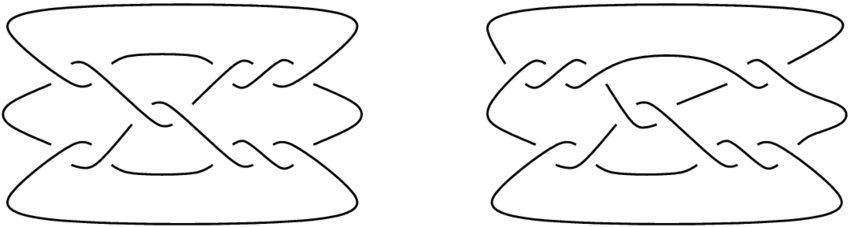
\includegraphics[width=10cm]{Images/The-Kinoshita-Terasaka-knot-left-and-Conway-mutant-right.png}
			\caption{O nó de Kinoshita-Terasaka (à esquerda) e o nó de Conway (à direita)}
		\end{center}
	\end{figure}
	\par\vspace{0.3cm} Recentemente, foi mostrado (\cite{Piccirillo}) que o nó de Conway (um nó descoberto por J.H. Conway meio século atrás), não é \textit{slice}. Essa propriedade, ser \textit{slice}, basicamente significa que esse nó é uma fatia de um nó em dimensão maior. Saber se um dado nó é \textit{slice} é uma das primeiras perguntas feitas a respeito de nós em espaços de dimensões maiores, e para todos os milhares de nós com $12$ cruzamentos ou menos essa pergunta já havia sido respondida, com exceção de um nó: o de Conway, com $11$ cruzamentos, que perdurou por décadas.
	\par\vspace{0.3cm} A dificuldade de responder se o nó de Conway era \textit{slice} ou não se devia ao fato de que ele é muito parecido com outro nó: o de Kinoshita-Terasaka. De fato, esses nós são ditos \textbf{mutantes}, pois é possível obter um do outro a partir de uma \textbf{mutação} (uma operação em um nó). Por ser muito parecido com o nó de Kinoshita-Terasaka, o nó de Conway conseguia escapar e evitar todos os invariantes utilizados para detectar nós que não fossem \textit{slice}. 
	\par\vspace{0.3cm} Antes de continuar com as propriedades dos polinômios de Alexander e Jones, seja $K$ um nó (ou \textit{link}) orientado. Se invertermos a orientação de $K$, obtemos um novo nó $\overline{K}$. Podemos supor que $K$ é o fecho da trança
	$\beta = \sigma_{i_1}^{\varepsilon_1}\sigma_{i_2}^{\varepsilon_2}\cdots\sigma_{i_k}^{\varepsilon_k}$. Daí, pelo item 2 da Proposição \eqref{representacao no espelhado}, $\overline{K}$ é o fecho da trança $\overline{\beta} = \sigma_{i_k}^{\varepsilon_k}\sigma_{i_{k-1}}^{\varepsilon_{k-1}}\cdots\sigma_{i_1}^{\varepsilon_1}$. 
	\begin{prop}
		\label{polinomio de Alexander para nos invertidos}
		Com os nós $K$ e $\overline{K}$ definidos acima, temos
		\begin{equation*}
		\Delta_{\overline{K}}(t) \doteq \Delta_K(t)
		\end{equation*}
	\end{prop}
	\begin{proof}
		Considere o homomorfismo $\varphi_n^\ast: B_n\to M(n, \mathbb{Z}[t,t^{-1}])$ definido anteriormente. Se $\beta=\sigma_{i_1}^{\varepsilon_1}\sigma_{i_2}^{\varepsilon_2}\cdots\sigma_{i_k}^{\varepsilon_k}$, então
		\begin{equation*}
		\varphi_n^\ast(\overline{\beta}) = \varphi_n(\sigma_{i_k}^{\varepsilon_k})^T\cdots\varphi_n(\sigma_{i_1}^{\varepsilon_1})^T = (\varphi_n(\sigma_{i_1}^{\varepsilon_1})\cdots\varphi_n(\sigma_{i_k}^{\varepsilon_k}))^T = \varphi_n(\beta)^T
		\end{equation*}
		
		\par\vspace{0.3cm} logo
		\begin{equation*}
		\det[\varphi_n^\ast(\overline{\beta}) - I_n]_{1,1} = \det[\varphi_n(\beta)^T - I_n]_{1,1} = \det[\varphi_n(\beta) - I_n]_{1,1}
		\end{equation*}
		\par\vspace{0.3cm} Portanto,
		\begin{equation*}
		\Delta_{\overline{K}}(t) \doteq \Delta_K(t)
		\end{equation*}
	\end{proof}
	\par\vspace{0.3cm} Com isso, concluímos que o polinômio de Alexander não é forte o bastante para detectar se um nó é invertível ou não (i.e., se é igual ao seu inverso), pois mostramos que o polinômio de Alexander é o mesmo para um nó $K$ e seu inverso $\overline{K}$. Além disso, como mostraremos a seguir, o polinômio de Alexander também falha em determinar se um nó é aquiral (i.e., se é igual a sua imagem espelhada) ou não. 
	\begin{prop}
		\label{polinomio de Alexander para nos espelhados}
		Sejam $K$ um nó (ou link) orientado e $K^\ast$ a imagem espelhada de $K$. Então,
		\begin{equation*}
		\Delta_K(t)\doteq\Delta_{K^\ast}(t)
		\end{equation*} 
	\end{prop}
	\begin{proof}
		Suponha que $K$ é representado como o fecho de uma trança $\beta$ de $n$ cordas. Então, o fecho de $\beta^{-1}$ representa o nó $\overline{K}^{\ast}$, que é a imagem espelhada de $K$ com orientação invertida (isso se deve ao item 1 da Proposição \eqref{representacao no espelhado}). Contudo, pelo Lema \eqref{lema Alexander},
		\begin{equation*}
		\Delta_K(t) \doteq \det[\varphi_n(\beta) - I_n]_{1,1} = \frac{1}{(1+t+\cdots+t^{n-1})}\det(\Lambda(t) - I_{n-1})
		\end{equation*}
		\par\vspace{0.3cm} e
		\begin{equation*}
		\Delta_{\overline{K}^{\ast}}(t) \doteq \det[\varphi_n(\beta^{-1}) - I_n]_{1,1} = \frac{1}{(1+t+\cdots+t^{n-1})}\det(\Lambda(t)^{-1} - I_{n-1})
		\end{equation*}
		\par\vspace{0.3cm} Note que
		\begin{align*}
		\det(\Lambda(t)^{-1} - I_{n-1}) &= \det(\Lambda(t)^{-1})\det(I_{n-1} - \Lambda(t)) \\
		&= -\det(\Lambda(t)^{-1})\det(\Lambda(t) - I_{n-1}) \\
		&\doteq \det(\Lambda(t)^{-1})(1+t+\cdots+t^{n-1})\Delta_K(t) 
		\end{align*}
		\par\vspace{0.3cm} e
		\begin{align*}
		\det(\Lambda(t)^{-1}) = \det( S^{-1}\varphi_n(\beta)^{-1}S ) = \det(\varphi_n(\beta)^{-1}) = (-t)^{\alpha}
		\end{align*}
		\par\vspace{0.3cm} em que a última igualdade segue de \eqref{det Burau de beta} e sendo $\alpha = l(\beta^{-1})$. Portanto, 
		\begin{equation*}
		(1+t+\cdots+t^{n-1})\Delta_{\overline{K}^{\ast}}(t)\doteq t^{\alpha}(1+t+\cdots+t^n-1)\Delta_K(t)
		\end{equation*}
		\par\vspace{0.3cm} e, daí
		\begin{equation*}
		\Delta_{\overline{K}^{\ast}}(t) \doteq \Delta_K(t)
		\end{equation*}
		\par\vspace{0.3cm} Como $\overline{K}^{\ast}$ é o inverso de $K^\ast$, então pela Proposição \eqref{polinomio de Alexander para nos invertidos}, temos, finalmente
		\begin{equation*}
		\Delta_{K^\ast}(t) \doteq \Delta_K(t)
		\end{equation*}
	\end{proof}
	\par\vspace{0.3cm} A implicação das Proposições \eqref{polinomio de Alexander para nos invertidos} e \eqref{polinomio de Alexander para nos espelhados} é que o polinômio de Alexander não é forte o suficiente para detectar ou não se um dado nó é aquiral nem invertível. Por outro lado, para o polinômio de Jones valem resultados similares, mas mais fortes.
	\begin{theorem}
		\label{polinomio de Jones para nos espelhados e invertidos}
		Seja $K$ um nó (ou link) orientado e sejam $\overline{K}$ e $K^\ast$ os nós definidos a partir de $K$ nas Proposições \eqref{polinomio de Alexander para nos invertidos} e \eqref{polinomio de Alexander para nos espelhados}, respectivamente. Então,
		\begin{enumerate}
			\item $V_{\overline{K}}(t) = V_K(t)$ 
			\item $V_{K^\ast}(t) = V_K(t^{-1})$
		\end{enumerate}
	\end{theorem}
	\begin{proof}
		
	\end{proof}
	\par\vspace{0.3cm} Um corolário imediato do Teorema \eqref{polinomio de Jones para nos espelhados e invertidos} é o seguinte.
	\begin{corollary}
		\label{simetria polinomio de Jones}
		Todo nó $K$ cujo polinômio de Jones $V_K(t)$ não é \textit{palindrômico} (i.e., simétrico sob a mudança de $t$ por $t^{-1}$) é \textit{quiral}, ou seja, distinto de sua imagem espelhada.
	\end{corollary}
	\par\vspace{0.3cm} Portanto, podemos usar o polinômio de Jones para detectar quando um nó (ou \textit{link}) \textbf{não} é aquiral. Contudo, o polinômio de Jones não é suficientemente forte para determinar o contrário. De fato, nós quirais para os quais $V_{K^\ast}(t) = V_K(t)$ foram encontrados. Por exemplo, o fecho da trança de $4$ cordas $\beta = \sigma_1^3\sigma_3\sigma_2^{-1}\sigma_3\sigma_1^{-2}\sigma_2^{-1}$ é quiral, mas 
	\begin{equation*}
	V_{\widetilde{\beta}^{-1}}(t) = t^{-3} - t^{-2} + t^{-1} - 1 + t - t^2 + t^3 = V_{\widetilde{\beta}}(t)
	\end{equation*}
	\par\vspace{0.3cm} De modo similar ao polinômio de Alexander, se tomarmos um gerador $\sigma_p$ de $B_n$ e uma trança $\beta\in B_n$, temos
	\begin{equation*}
	\frac{1}{t}V_{\widetilde{\beta\sigma_p}}(t) - tV_{\widetilde{\beta\sigma_p^{-1}}}(t) = \left( \frac{1}{\sqrt{t}} - \sqrt{t}\right)V_{\widetilde{\beta}}(t)
	\end{equation*}
	\section{O grupo de Alexander}
	\hspace{12pt} Um outro invariante de nós é o chamado \textit{grupo de Alexander}, denotado por $A(K)$, $K$ um nó. O grupo de Alexander de um nó é um grupo abeliano definido em termos das regiões de um nó.
	\par\vspace{0.3cm} Suponha que a projeção de um nó tenha $n$ cruzamentos. Daí, essa projeção tem $n+2$ regiões (contando o ``lado de fora'' como uma região). Os geradores de $A(K)$ são exatamente essas $n+2$ regiões. Há também $n$ relações, uma para cada cruzamento.
	\par\vspace{0.3cm} Se as regiões em volta de um cruzamento são $a,b,c,d$, com $a,b$ de um lado do cruzamento e $c,d$ do outro, a relação correspondente é $a+b=c+d$.
	\par\vspace{0.3cm} Por exemplo, o nó figura oito abaixo tem grupo de Alexander dado por 
	\begin{align*}
	A(K) = [a,b,c,d,e,f \ \vert \ a+b=c+f,\ a+d=b+c,\ a+f=d+e,\ c+d=e+f] 
	\end{align*}
	\par\vspace{0.3cm} que, escrito em forma matricial, se torna
	\begin{align*}
	\begin{bmatrix}
	1 & 1 & -1 & 0 & 0 & -1 \\
	1 & -1 & -1 & 1 & 0 & 0 \\
	1 & 0 & 0 & -1 & -1 & 1 \\
	0 & 0 & 1 & 1 & -1 & -1 
	\end{bmatrix}\cong\mathbb{Z}\oplus\mathbb{Z}\oplus\mathbb{Z}_5
	\end{align*}
	
	\begin{figure}[H]
		\label{exemplo grupo Alexander}
		\begin{center}
			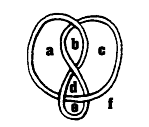
\includegraphics[width=4cm]{Images/exemplo_grupo_alexander.png}
		\end{center}\caption{Nó figura oito e suas regiões}
	\end{figure}
	\par\vspace{0.3cm} Outro invariante também relacionado às regiões de um nó é o \textit{número de Alexander}. Ele é análogo ao grupo de Alexander, mas agora vamos numerar as regiões ao invés de nomeá-las. Antes de tudo, a notação usada é a seguinte:
	\begin{center}
		\begin{tabular}{ccc}
			$a$ & $\vert$ & $b$ \\
			\hline 
			$c$ & $\vert$ & $d$
		\end{tabular}
	\end{center}
	\par\vspace{0.3cm} As duas linhas representam as duas cordas de um cruzamento e as letras $a,b,c,d$ representam as regiões em volta de tal cruzamento. Assim como antes, devemos ter $a+b=c+d$. Por exemplo, se tivermos
	\begin{center}
		\begin{tabular}{ccc}
			3 & $\vert$ & 5 \\
			\hline 
			1 & $\vert$ & ?
		\end{tabular}
	\end{center}
	\par\vspace{0.3cm} então devemos ter $?=7$, uma vez que $5+3=1+7$.
	\par\vspace{0.3cm} Para começar, começamos colocando $0$, $0$ e $1$ em três regiões em volta de um cruzamento. A região restante será numerada com $1$ ou $-1$, o que for necessário para satisfazer a igualdade.
	\begin{align*}
	\begin{array}{ccc}
	0 & \vert & 0 \\
	\hline 
	1 & \vert & -1
	\end{array} \ \text{ ou } \ 
	\begin{array}{ccc}
	0 & \vert & 1 \\
	\hline 
	0 & \vert & 1
	\end{array}
	\end{align*} 
	\par\vspace{0.3cm} Na prática, é uma boa ideia começar a numeração com a região de fora e ir preenchendo todas as regiões. Por exemplo, para o nó de trevo
	\begin{figure}[H]
		\label{no de trevo negativo}
		\begin{center}
			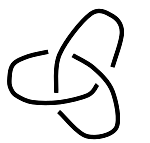
\includegraphics[width=2.5cm]{Images/no_de_trevo_negativo.png}
		\end{center}
	\end{figure}
	\par\vspace{0.3cm} começamos com a região de fora
	\begin{figure}[H]
		\label{no de trevo preenchendo}
		\begin{center}
			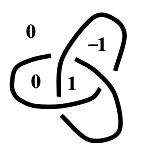
\includegraphics[width=2.5cm]{Images/no_de_trevo_preenchendo.png}
		\end{center}
	\end{figure}
	\par\vspace{0.3cm} e balanceamos o cruzamento à direita, da seguinte forma: lembre que toda a região de fora é $0$, então de um lado temos $-1+0=-1$. Logo, a última região deve ser $-2$, uma vez que $-1+0=1+(-2)$. Daí, obtemos
	\begin{figure}[H]
		\label{no de trevo preenchido}
		\begin{center}
			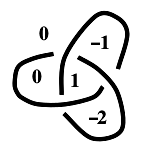
\includegraphics[width=2.5cm]{Images/no_de_trevo_preenchido.png}
		\end{center}
	\end{figure}
	\par\vspace{0.3cm} Note, contudo, que no cruzamento inferior à esquerda, temos $0+1=-2+0$, i.e., $3=0$. Isso não seria verdade em aritmética ordinária, mas em aritmética modular essa igualdade é verdade para módulo $3$. De fato, o número de Alexander é o maior módulo que faz com que o último cruzamento fique balanceado. Nesse caso, é $3$. Então, note que se o último cruzamento tem equação $n=0$ para algum $n$ positivo, então $n$ é o nosso número de Alexander. 
	\par\vspace{0.3cm} Para o nó figura oito, temos
	\begin{figure}[H]
		\label{no de oito preenchido}
		\begin{center}
			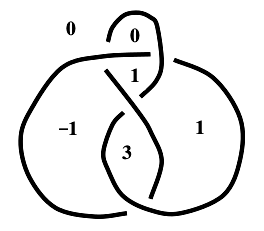
\includegraphics[width=4.5cm]{Images/no_de_oito_preenchido.png}
		\end{center}
	\end{figure}
	\par\vspace{0.3cm} O último cruzamento (inferior) nos dá $3+1=-1+0$, ou seja, $5=0$. Logo, o número de Alexander para o nó figura oito é $5$.
	\par\vspace{0.3cm} O número de Alexander para o nó de trevo é $3$, e para o nó figura oito, $5$. Logo, o nó de trevo não é equivalente ao nó figura oito, como esperado.
	\par\vspace{0.3cm} Para ganhar um pouco mais de intuição e certeza de que o número de Alexander é um invariante (não demonstraremos aqui), observe as seguintes figuras.
	%
% 	\begin{figure}[H]
% 		\centering
% 		\begin{subfigure}[t]{0.5\textwidth}
% 			\centering
% 			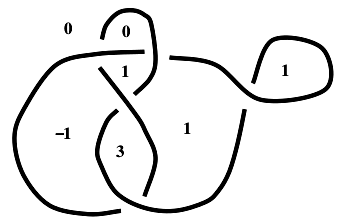
\includegraphics[width=3cm]{Images/no_de_oito_com_cruzamento_extra.png}
% 			\caption{$\Omega_1$}
% 			\label{numero de Alexander e Reidemeister 1}
% 		\end{subfigure}%
% 		~
% 		\begin{subfigure}[t]{0.5\textwidth}
% 			\centering
% 			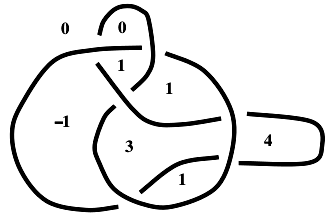
\includegraphics[width=3cm]{Images/no_de_oito_com_corda_por_baixo.png}
% 			\caption{$\Omega_2$}
% 			\label{numero de Alexander e Reidemeister 2}
% 		\end{subfigure}
% 		\caption{O nó figura oito submetido aos movimentos de Reidemeister 1 e 2}
% 	\end{figure}
	%
	%
	\begin{figure}[H]
        \centering
        \subfloat[$\Omega_1$]{\label{numero de Alexander e Reidemeister 1}{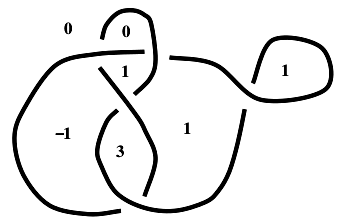
\includegraphics[width=3cm]{Images/no_de_oito_com_cruzamento_extra.png}}}\hfill
        \subfloat[$\Omega_2$]{\label{numero de Alexander e Reidemeister 2}{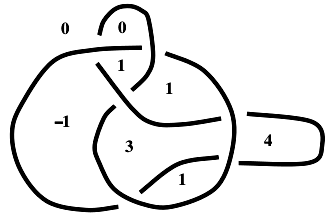
\includegraphics[width=3cm]{Images/no_de_oito_com_corda_por_baixo.png}}}
        \caption{O nó figura oito submetido aos movimentos de Reidemeister 1 e 2}
    \end{figure}
	%
	\par\vspace{0.3cm} Note que em ambos os diagramas acima o número de Alexander não mudou: tanto para a Figura \ref{numero de Alexander e Reidemeister 1} quanto para a Figura \ref{numero de Alexander e Reidemeister 2} o último cruzamento continua tendo equação $3+1=-1+0$, i.e., $5=0$, e o número de Alexander continua sendo $5$.
	\par\vspace{0.3cm} O exemplo acima esboça a ideia para se demonstrar que o número de Alexander de fato é um invariante: basta mostrarmos que os movimentos de Reidemeister dos tipos I e II não alteram o número de Alexander.
	\par\vspace{0.3cm} Um último exemplo que vale a pena mencionar é o preenchimento do seguinte nó
	\begin{figure}[H]
		\begin{center}
			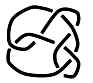
\includegraphics[width=3cm]{Images/no_exemplo_travado.png}
		\end{center}
	\end{figure}
	\par\vspace{0.3cm} Considere que começamos o preenchimento da seguinte forma
	\begin{figure}[H]
		\begin{center}
			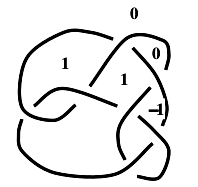
\includegraphics[width=4cm]{Images/no_preenchimento_incompleto.png}
		\end{center}
	\end{figure}
	\par\vspace{0.3cm} Começando no cruzamento superior, chegamos em um impasse: não há como seguir preenchendo, pois todo cruzamento tem pelo menos duas regiões não preenchidas. Contudo, se começarmos o preenchimento da seguinte forma
	\begin{figure}[H]
		\begin{center}
			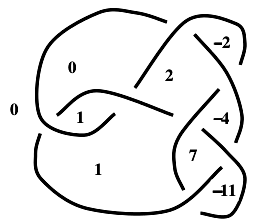
\includegraphics[width=4cm]{Images/no_preenchimento_completo.png}
		\end{center}
	\end{figure}
	\par\vspace{0.3cm} conseguimos finalizá-lo, obtendo, no último cruzamento, $1+7=-11+0$, i.e., $19=0$. Logo, o número de Alexander para esse nó é $19$.
	\par\vspace{0.3cm} Como pudemos perceber, às vezes podemos contornar um impasse sendo um pouco mais espertos. Contudo, esse nem sempre é o caso. Existem nós mais complicados para os quais, independentemente do que façamos, é impossível proceder. Ainda assim, é possível encontrar o número de Alexander, mas são necessárias técnicas mais avançadas.